 \documentclass[
 a4paper,
12pt,			% font size
headsepline
]{report}

\usepackage[utf8]{inputenc}		% Pour afficher les caracteres internationaux
\usepackage[T1]{fontenc}			% Pour l'encodage de caracteres
\usepackage[french]{babel}

\usepackage{lmodern} % Pour changer le pack de police
\usepackage{makeidx}
\usepackage{layout}

\usepackage{graphicx}   % For images 
\usepackage{subcaption} % for multiple image caption

\usepackage{listings} 	% for Code listing
\usepackage{csquotes}

\usepackage[table,xcdraw]{xcolor}
\usepackage{array}

%----------------------------------------------------------------------------------------
%	CodeListing
%----------------------------------------------------------------------------------------

\definecolor{commentcolor}{rgb}{0,0.6,0}
\definecolor{codegray}{rgb}{0.5,0.5,0.5}
\definecolor{codepurple}{rgb}{0.58,0,0.82}
\definecolor{backcolour}{rgb}{0.95,0.95,0.92}
\definecolor{black}{rgb}{0.0,0.0,0.0}
\definecolor{primary}{rgb}{0,0.6,0}
\definecolor{secondary}{rgb}{0,0.6,0}

\lstdefinestyle{JSON}{
	string=[s]{"}{"},
	stringstyle=\bfseries\color{black},
	comment=[l]{:},
	commentstyle=\color{secondary},
	breakatwhitespace=false,
    breaklines=true,                 
    captionpos=b,                    
    keepspaces=true,                 
    numbers=left,                    
    numbersep=5pt,                  
    showspaces=false,                
    showstringspaces=false,
    showtabs=false,                  
    tabsize=2
} 

 
\lstdefinestyle{cypher}{
    backgroundcolor=\color{backcolour},   
    commentstyle=\color{commentcolor},
    keywordstyle=\bfseries\color{primary},
    keywordstyle = [2]{\color{secondary}},
    keywordstyle = [3]{\color{codepurple}},
    morekeywords = [1]{MATCH, AllShortestPaths, WHERE, ALL, IN},
    morekeywords = [2]{WITH,EXTRACT,RETURN,AND, AS},
    morekeywords = [3]{EndNode,StartNode,RELATIONSHIPS},
    numberstyle=\tiny\color{codegray},
    string=[s]{\{}{\}},
  	comment=[l]{},
	stringstyle=\bfseries\color{black},
    stringstyle=\color{codepurple},
    basicstyle=\footnotesize,
    breakatwhitespace=false,         
    breaklines=true,                 
    captionpos=b,                    
    keepspaces=true,                 
    numbers=left,                    
    numbersep=5pt,                  
    showspaces=false,                
    showstringspaces=false,
    showtabs=false,                  
    tabsize=2
}

\lstset{style=Cypher}


% Bibliography 
\usepackage[backend=bibtex,sorting=none]{biblatex}
\addbibresource{bibliographie}


%----------------------------------------------------------------------------------------
%	MARGIN SETTINGS
%----------------------------------------------------------------------------------------

\usepackage[top=1in, bottom=1in, left=1in,right=1in,footskip=0.5in,
headheight=15.5pt]{geometry} 

% ========= FOR LINKS ============= % 
\usepackage{color}   %May be necessary if you want to color links
\usepackage{hyperref}	% clickable links 
\hypersetup{
    colorlinks=true, %set true if you want colored links
    linktoc=all,     %set to all if you want both sections and subsections linked
    linkcolor=black,  %choose some color if you want links to stand out
}

%----------------------------------------------------------------------------------------
%	TEXT STYLES
%----------------------------------------------------------------------------------------
\usepackage{float} %used for figure placement with H as a parameter
\usepackage{setspace}
\usepackage{float}
\usepackage{enumerate}

\usepackage[font=small,labelfont=bf]{caption}
\def\figurename{\textbf{Figure }}

%----------------------------------------------------------------------------------------
%	HEADERS/FOOTERS
%----------------------------------------------------------------------------------------

\usepackage{scrlayer-scrpage}

\automark{chapter}
\automark*{section}
\clearpairofpagestyles
\ihead{\headmark}
\ohead{\pagemark}
%\renewcommand{\headrulewidth}{0.4pt}
%\renewcommand{\footrulewidth}{0.4pt}

\ifoot{}% Inner footer
\ofoot{}% Outer footer

% Pour supprimer le footer en présence des footnotes
\newcommand{\FancyFootNote}[1]{
    \footnote{#1}
%    \thispagestyle{plain_nofoot} %change pagestyle for this page only.
}

% ====================================================%
% =================== DOCUMENT ======================%
% ====================================================%
\pagenumbering{roman} %numbering before main content starts

\title{Projet Fin Etude}
\author{Serious Person 1, Serious Person 2}
\date{\today}

\makeindex

\begin{document}	
\maketitle
%	\layout			% verifier dimensions/ structure de la page

%\pagestyle{fancy}	

\chapter*{Abstract} 

%\pagestyle{plain}	


%----------------------------------------------------------------------------------------
%	LIST OF CONTENTS/FIGURES/TABLES PAGES
%----------------------------------------------------------------------------------------

\pdfbookmark[0]{Contents}{contents}
\tableofcontents % Prints the main table of contents

\listoffigures % Prints the list of figures

%\listoftables % Prints the list of tables
	
%----------------------------------------------------------------------------------------
%	REPORT CONTENT - CHAPTERS
%----------------------------------------------------------------------------------------

\pagenumbering{arabic} %reset numbering to normal for the main content
	
% Chapitre1/intro
\renewcommand\labelitemi{$\bullet$}
\renewcommand\labelitemii{$\circ$}
\chapter{Introduction générale}
\newpage	
\section{Motivation}
La population mondiale connaît une très forte croissance depuis 1900. 
Il y avait 1,5 milliard d'hommes au début du siècle, 2,5 milliards en 1950 , et aujourd'hui en 2018: 7,4 milliards. 
Les villes se sont développées, au cours des 19e et 20e siècles, sur des carrefours de communication, des fleuves ou sur des littoraux. Des banlieues se sont également développées autour des grandes villes. 
Avec ce développement, un réseau de transport public a été nécessaire pour permettre de lier les éléments essentiels de ces villes. 
Mais cette demande croissante de transport a engendré de nouveaux problèmes. Parmi eux, le fait que les usagers nécessitent souvent un moyen pour s'orienter et se renseigner.

L'informatique a apporté plusieurs solutions à ce problème. Il existe en effet plusieurs moyens de visualisation cartographique.
On cite OpenStreetMap et Google Maps comme exemple, qui permettent la manipulation et visualisation de données géographiques du monde entier, de tracer des itinéraires entre deux points et d'aider les utilisateurs à marquer et trouver leur magasins, hôtel ou un autre lieu favori.
Cependant, ces outils ne proposent généralement qu'un seul moyen de transport. De plus, certaines de ces fonctionnalités ne sont pas adaptées pour tous les pays, voire non disponibles.
Ajouté à ça un nombre immense de lignes de bus, par example, avec des noms très peu significatifs et une organisation aléatoire des lignes qui changent fréquemment: des facteurs contribuant encore plus à la confusion des usagers. 


Ces raisons font que trouver un chemin optimal faisant bon usage de différents moyens de transport pour une personne est une tâche bien difficile, car ça demande principalement une connaissance parfaite de toute la ville, chose qui est impossible notamment pour un touriste.
Le choix du chemin dépend aussi de plusieurs facteurs : la situation et les préférences de chaque personne, ainsi que le jour du trajet, l'heure et la météo.
Par exemple, un usager peut choisir habituellement de marcher vers un arrêt de tramway et puis le prendre jusqu'à sa destination, mais préfère, en jour de pluie ou suite à défaut de pouvoir marcher, de prendre deux bus avec un chemin plus long.

Notre but est donc de créer un outil qui aide à cette décision, qui sera ensuite adapté à la ville d’Oran.

\section{Intérêt et avantages}
Offrir un guide de transport évolué a pour apport :
\begin{itemize}
	\item Gain considérable de temps, de transport et réduction de dépenses.
	\item Assurer un meilleur respect d'horaire et d'itinéraires de la part des entreprises de transport, et ainsi avoir plus de confiance de la part des utilisateurs.
	\item Encourager plus de citoyens à utiliser les transports communs.
	\item Améliorer la circulation en ville en diminuant le nombre d'utilisateurs de véhicules personnel et ainsi réduire les embouteillages.
	\item Meilleure expérience aux touristes et visiteurs.
\end{itemize}

\section{Problématique}

La création d'un outil qui aide à cette décision présente plusieurs problématiques, avant de commencer le projet, nous sommes amenés à répondre aux questions suivantes :
\begin{itemize}
	\item Quels sont ces différents facteurs et critères à considérer lors de ce choix ?
	\item Quelles sont les différents usagers des transports communs, et quel est le besoin de chaque profile ?
	\item Quelles sont les différentes difficultés et contraintes qui peuvent affecter ce choix?
	\item Peut on offrir une solution informatique évoluée pour assister à ce choix ? Si oui : 
	      \begin{itemize}
	      	\item Comment représenter un réseau routier d'une ville comme Oran, et contenant plusieurs moyens de transport ?
	      	\item Comment calculer un chemin sur ce réseau, et comment déterminer un chemin optimal ?
	      	\item Comment inclure les différentes préférences et circonstances de chaque utilisateur ?
	      	\item Comment présenter cette solution aux usagers de manière simple et efficace ?
	      \end{itemize}
\end{itemize}
			
\section{Applications similaires}			
\subsection{RATP}
L'application RATP a été développée 2010 dans le but d'injecter du réseau social dans le réseau souterrain. Aujourd'hui c'est le compagnon de transport pour Paris et l'ile de France.
Parmi les services qu'elle propose, on cite:
\begin{itemize}
	\item La possibilité de consulter les horaires de passages des différents moyens de transport public desservant Paris et ses environs. 
	\item Permet de retrouver les stations ou les arrêts autour de l'endroit où se trouve l'utilisateur grâce à la géolocalisation.
\end{itemize}
Un avantage particulier avec RATP est le fait qu'il peut être paramétré de manière à émettre des alertes en cas de perturbations ou éventuels retards sur une ligne particulière.
	
\subsection{CityMapper}
CityMapper est une application de transports en commun qui a été lancé à Londres en 2011.
Elle propose 3 modes d'utilisation : 
\begin{itemize}
	\item Découvrir de tous les modes de transports en commun dans cette ville.
	\item Obtenir les différents moyens pour arriver à la destination souhaitée.
	\item Comparer le temps de chaque trajet.
\end{itemize}

CityMapper couvre en ce moment 36 villes dont Londres, Berlin, Tokyo, Paris et New York...etc.  Un de ses avantages est la possibilité de prévoir un trajet en avance et de le télécharger pour qu'il soit disponible hors connexion.

\section{Solution proposée}
Au moment de rédiger ce mémoire, aucune application n'offre ce service en Algérie. ***

De ce fait, nous proposons de développer une application Web full-REST qui proposera les fonctionnalités suivante : 

\begin{itemize}
	\item Calculer un chemin entre deux lieux saisis par l'utilisateur.
	\item Proposer un chemin optimal faisant usage de plusieurs moyens de transport publique, tout en donnant la main à l'utilisateur pour choisir les moyens désirés.
	\item Prendre en compte la possibilité de marche dans les chemins suggérés.
	\item Se baser sur différents critères dans ce choix, nous prendrons les 04 critères suivants : 
	\begin{itemize}
		\item Minimum de temps.
		\item Minimum de marche.
		\item Minimum de correspondance.
		\item Minimum de cout.
	\end{itemize}	 
\end{itemize}

Ce projet sera composé de 04 parties :
\begin{description}
	\item[Conception de base de donnée: ] Nous étudierons le problème pour enfin proposer une bonne représentation des données que nous pourrons facilement utiliser dans la recherche de chemin.
	( *** Est ce qu'on cite la bdd orienté graphe ici ? *** )
	
	\item[Service Web: ] En ce moment, les Services Web sont une tendance sur le Web, presque indispensable dans toute application non triviale: Nous commencerons donc par créer une API REST complète de l'application afin qu'elle soit facilement extensible et portable sur différentes plateformes par la suite.
	
	\item[Interface Administrateur: ] Implémenter une application indépendante qui va faciliter la  communication avec l'API pour l'ajout et modification des lignes de transport et autres informations nécessaire à l'application.
	
	
	\item[Interface Web: ] Implémenter une Application Web client afin de visualiser les fonctionnalités de l'API.
\end{description}

Vu le grand nombre de fonctionnalités et la complexité de cette problématique, nous limiterons la version initiale de l'application à un premier algorithme de recherche simple mais applicable sur la ville d'Oran.

L'architecture de l'application devra être suffisamment flexible pour pouvoir améliorer la recherche de chemin, et ajouter progressivement des améliorations ou de nouvelles critères.
	 
		 
\newpage
\section{Plan du rapport}

**Parler des points suivants 
\begin{itemize}
\item On présentera tout au long du Chapitre 2 ce qu'est un service Web, ses caractéristiques et avantages. 
Nous explorerons ensuite deux manières concurrentes pour implémenter des Services Web : SOAP et REST. 
Nous débattrons brièvement les points forts de chacun afin de justifier notre décision d'utiliser REST.

\item Chapitre 3 : c'est compliqué.

\item Nous présenterons ensuite dans le chapitre 4 les differentes technologies qu'on a utilisé, ainsi qu'un aperçu des représentations utilisée et des détails implémentations. ***qui seront accompagnées par des captures d'écran décrivant le fonctionnement de l'application.**
\item Nous parlerons enfin dans le chapitre 5 sur les differentes perspectives et futur stuff
\end{itemize}
%Chapitre 2	
\chapter{Les Services Web}
\newpage
\section{Introduction} 
\paragraph{(Laisser l'introduction et conclusion à la fin)}
\begin{itemize}
	\item Web passé de centré interaction utilisateur à plus d'interaction entre applications..
	\item avant les services web
\end{itemize}
		
\section{Avant les services web}
Parler brièvement des prédecesseurs (COBRA, DCOM) middlewares et protocoles, XML-RPC.\newline
		
Vers les années 90s, les technologies Web et les technologies des systèmes distribuées ont commencé à gagner en popularité. Les technologies Web étaient principalement conçues pour envoyer des informations d'utilisateur à un autre, en HTML par example. Les technologies de systèmes distribués, cependant, étaient principalement conçues pour connecter des ordinateurs, ou plus spécifiquement des applications exécutées sur ces machines, et donc leurs permettre de s'échanger des informations ou collaborer sur des tâches.
Chacune de ces deux technologies avaient des objectifs différents, et évoluaient vers un chemin différent. Ainsi, les Services Web sont apparu avec but de rassembler ces deux technologies sur un seul objectif commun reliant les deux.\cite{W3Road}

\section{Définition}
Un Service Web est un programme dynamique qui utilise le schéma Client-Serveur pour permettre la communication et l'échange de données entre des applications à travers un réseau (Internet par exemple).
Il utilise un système de messagerie standard\FancyFootNote{Un protocole standard est un protocole formalisé (fixé) accepté par une autorité (comme la W3C) ou la plupart des parties qui l'implémentent.} comme XML mais n'est lié à aucun système d'exploitation ou langage de programmation.

Quelques définitions officielles :
\begin{enumerate}
	\item W3C :
	      Un Service Web est un composant logiciel conçu pour permettre l'interaction interopérable entre machines à travers un réseau. Il a une interface décrite en un format compris par une machine (Spécifiquement WSDL). Les autres systèmes interagissent avec le Service Web d'une manière définie par sa description en utilisant des messages SOAP, généralement transmis en utilisant HTTP avec un XML sérialisé en parallèle avec d'autres Standard du Web.\cite{W3}
	\item Wikipedia : Un service web (ou service de la toile) est un protocole d'interface informatique de la famille des technologies web permettant la communication et l'échange de données entre applications et systèmes hétérogènes dans des environnements distribués. Il s'agit donc d'un ensemble de fonctionnalités exposées sur internet ou sur un intranet, par et pour des applications ou machines, sans intervention humaine, de manière synchrone ou asynchrone. Le protocole de communication est défini dans le cadre de la norme SOAP dans la signature du service exposé (WSDL). Actuellement, le protocole de transport est essentiellement HTTP(S).\cite{Wikipedia}
\end{enumerate}

\section{Principe et objectifs}
\subsection{Pourquoi les services Web ?}
Les services web ont été conçus pour permettre l'interaction interopérable entre machines à travers un réseau, en d'autre termes, permettre à différents systèmes de fonctionner et communiquer entre eux.\newline
Puisque différentes applications peuvent être écrites en différents langages et architectures, et sont souvent ramenées à subir plusieurs changements, l’interaction directe entre ces applications est souvent difficile voire pas possible, un service web implémenté pour une application ou ressource offre donc un moyen compréhensible par les autres machines d'accéder aux services de cette application et ce, indépendamment de la technologie implémentée par cette application.
\cite{refTutorialPointsWS}
\subsection{Fonctionnement général d'un Service Web}
Un service web est un agent réalisé par un fournisseur de service, cet agent joue le rôle d'un intermédiaire entre ce service et les demandeurs extérieurs, ou clients, qui communiquent à travers leur \emph{agent de requête}. 
\newline			
Un service web permet donc de recevoir des messages d'un agent de requête, qu'il traduit ou transmit au service dans un format compris par le fournisseur du service.\newline La figure \ref{Generalite_figure} résume le rôle de ces différents acteurs.
\begin{figure}[h]
	\center
	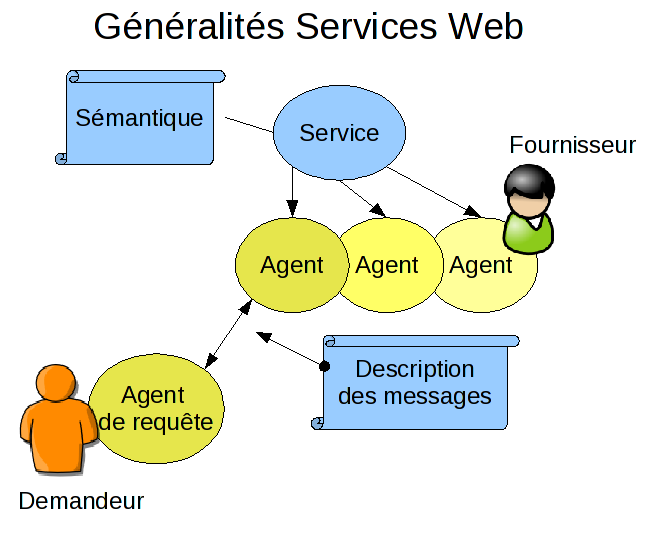
\includegraphics[scale=0.5]{img/Whatisaserviceweb.png}
	\caption{Generalités Services Web}		
	\label{Generalite_figure}
	\centering
\end{figure}						
\newline
Dans la figure \ref{Generalite_figure}, l'agent de requête et l'agent du service utilisent le même format de message, basé sur ensemble de standards et de protocoles ouverts déjà existants, tel que le XML.
Ces protocoles sont implémentés par défaut (ou faciles à intégrer) dans la majorité des technologies, ce qui permet la communication entre différentes applications sans contraintes majeures. 
	
Ce système est réalisé grâce à plusieurs technologies, les plus connus étant les Services Web type SOAP et les Services Web type REST, détaillés dans les parties 2.5 et 2.6 respectivement.
	
\subsection{L'architecture orientée services} 
L'architecture orientée services (Service Oriented Architecture, SOA) est style architectural qui vise à concevoir des services web extensibles et hautement réutilisables, et les rendre ensuite visibles et accessibles aux consommateurs.
				
On trouve trois acteurs majeurs dans une architecture SOA de service web :
\begin{itemize}
	\item \textbf{Service Provider} : 
	      C'est le fournisseur du service. il implémente le service et le rends disponible sur le réseau.
	\item \textbf{Service requester} :
	      C'est le consommateur (Client) de ce service. Il utilise un service web existant en ouvrant une connexion réseau et en envoyant des requêtes (par example des messages en XML).
	\item \textbf{Annuaire service registry} : 
	      C'est un annuaire de services. ce registre fournit un endroit central où les développeurs peuvent publier leur nouveau service web, ou trouver d'autres existants.\newline 
\end{itemize}

Les services Web emploient un ensemble de technologies qui ont été conçues en respectant une structure en couches sans être dépendantes entre elles. Cette pile, appelée "Pile de protocoles de services web", peut évoluer, mais elle est principalement formée de quatre couches : \cite{refTutorialPointsWS}
\begin{description}
	\item[Couche transport] : Cette couche est responsable du transport des messages échangés entre les applications, cette couche utilise généralement le protocole HTTP, mais d'autres tel que SMTP, FTP ou BEEP peuvent être utilisés.
	\item [Couche communication (Messaging)] : Cette couche est responsable de la représentation et formatage des messages échangés entre applications, et ceci afin d'assurer qu'ils soient compris par chaque extrémité. Cette couche utilise principalement XML (ou un dérivé de ce dernier comme XML-RPC et SOAP), mais peut aussi utiliser d'autres formats standard suivant l'architecture, Les services REST peuvent envoyer en simple texte, JSON ou XML par example.
	\item[Couche description de service] : Cette interface est responsable de la description de l'interface publique du Service Web, cette description est réalisée en utilisant le WSDL.\newline
	      \texttt{WSDL : (Web Services Description Language)} : c'est un langage de description standard basé sur XML, développé en jointure par Microsoft et IBM. Il permet de décrire différentes informations sur le Service Web tel que la liste de ses fonctions, comment interagir avec et les invoquer, les ports et protocoles utilisés...etc.
	\item[Couche découverte de service] : Cette couche est responsable de centraliser les services dans un registre commun, et fournir des fonctionnalités de recherche/publication de services web. Ce service est assuré par l'annuaire UDDI.\newline
	      \texttt{UDDI (Universal Description, Discovery and Integration)} : C'est un annuaire de services web, ce protocole, basé sur XML, comporte deux sections en WSDL : les descriptions de ces services et des définitions de ports pour manipuler et rechercher dans l'annuaire.
\end{description}
			
\subsection{Caractéristiques d'un Service Web}
Dans un Service Web complet on trouve les caractéristiques suivantes :\cite{refTutorialPointsWS}
\begin{itemize}
	\item Il ne dépends d'aucun Système ou langage.
	\item Il est accessible par un réseau (Internet/Intranet).
	\item Il dispose d'une interface publique permettant au clients d'invoquer des procédures ou méthodes sur des objets distants, l'annuaire du service contient la descriptions de ces fonctionnalités et comment les utiliser.
	\item Utilise un système de messagerie standard (souvent basés sur XML).
	\item Les fonctionnalités utilisées par le service sont regroupées en un nombre limité de \emph{gros grains} qui sont exposés ensuite au client et ainsi permettre une interaction plus simple avec le service. Par example, regrouper des fonctions de bas niveau (petites graines) en une seule fonction de haut niveau, et exposer celle ci sur le réseau.
	\item Son système est \emph{faiblement couplé} : Le consommateur de ce service n'est pas directement lié au service, ce service peut changer au fil du temps sans perturber le client, ou peut même disparaitre et le client trouvera un autre service en cherchant dans son annuaire.
\end{itemize}
		
%=================================================================
%=========================== PARTIE HTTP ==========================
%=================================================================
\newpage
\section{Le protocole HTTP}
Dans le modèle Client-serveur, les clients et les serveurs échangent des messages dans un modèle de messagerie de type requête-réponse : le client envoie une requête et le serveur renvoie une réponse.
Pour gérer ces messages et définir un format commun entre eux, on utilise le protocole HTTP.

\subsection{HTTP (Hyper Text Transfer Protocol)}
C'est un protocole qui décrit le contenu et la mise en forme des requêtes et des réponses échangées entre le client web et le serveur web. 
Lorsqu'un client, généralement un navigateur web, envoie une requête à un serveur web, il utilise un URL combinée avec un "verbe" HTTP pour spécifier le type de message et l'action que doit prendre le serveur sur une ressource.

\subsection{Methodes HTTP}
HTTP propose plusieurs verbes (ou méthodes), mais les plus importants sont : 
\begin{itemize}
	\item \textbf{GET} : Obtenir des données, un navigateur web envoie une requête GET au serveur web pour demander des pages HTML par example.
	\item \textbf{POST} : Envoyer des fichiers ou de données vers le serveur web, comme des données de formulaires.
	\item \textbf{PUT} : Envoyer des ressources ou du contenu vers le serveur web, similaire à POST mais utilisé principalement pour mettre à jour une ressource, PUT doit être idempotente : c'est à dire qu'envoyer plusieurs fois la même requête produit le même résultat que la première.
	\item \textbf{DELETE} : c'est une requête  qui supprime la ressource indiquée.
\end{itemize}

\subsection{HTTPS}
Le protocole HTTP est certes extrêmement flexible, mais il n'est pas sécurisé. Les messages de demande transmettent au serveur des informations en texte brut pouvant être interceptées et lues. Les réponses du serveur, généralement des pages HTML, ne sont pas chiffrées.
Pour une communication sécurisée via Internet, le protocole HTTPS (HTTP Secure) est utilisé. HTTPS utilise l'authentification et le chiffrement pour sécuriser les données pendant leur transfert entre le client et le serveur. HTTPS utilise le même processus de demande client-réponse serveur que le protocole HTTP, sauf que le flux de données est chiffré avec le protocole SSL (Secure Socket Layer) avant d'être transporté sur le réseau.

%=================================================================
%=========================== PARTIE SOAP ==========================
%=================================================================
\newpage
\section{Services web SOAP} 
\subsection{Le protocole SOAP}
SOAP (Simple object Access Protocol) est un protocole de communication standardisé par le W3C. 
Il définit un format pour l'envoi des messages (basé sur XML) sous forme d'enveloppe et de son contenu, qui peuvent être envoyés par divers protocoles de transport tel que HTTP et SMTP.
				
SOAP s'appuie donc sur des standards très connus, ce qui lui a donné une grande portabilité et interopérabilité comparé à ses prédécesseurs (COBRA, DCOM, JAVA RMI...etc).
				
\subsection{Structure de message SOAP}
Un message SOAP est un document XML contenant les éléments suivants : \cite{refTutorialPointsSOAP}
\begin{itemize}
	\item \textbf{Enveloppe} : Définit le début et fin du message, elle contient contient la spécification des espaces de désignation (namespace\FancyFootNote{Un namespace est un préfixe identifiant de manière unique la signification d'un terme pour éviter toute ambiguïté.}) et le codage des données. c'est un élément obligatoire.
	\item \textbf{Header (Entête)} : Contient des informations ou options supplémentaires pour le traitement du message comme l'encodage, elle est optionnelle.
	\item \textbf{Body ( Corps )} : Contient les données XML du message à transporter, un élément obligatoire.
	\item \textbf{Fault (Gestion d'erreurs)} : Fournit des informations sur les erreurs qui peuvent se produire au traitement de l'information, un élément qui peut être optionnel.
\end{itemize}
\begin{figure}[h]
	\begin{center}
		\includegraphics[scale=1]{img/soapmessagebody.png}
	\end{center}	
	\label{Structure message SOAP}
	\caption{Structure message SOAP}		
	\centering
\end{figure}			
Un message SOAP est un peu lourd, mais reste simple à comprendre et à utiliser, sa structure offre une fiabilité par rapport au format de données, ainsi qu'un moyen de gérer les erreurs grâce au SOAP Fault.
\newpage
\subsection{Inconvenients}
Bien que SOAP soit une solution standardisée pour l'accès aux Services Web, on peut noter certains inconvénients :
\begin{itemize}
	\item \textbf{Lourdeur :} L'utilisation d'XML et la structure des messages SOAP est assez verbeuse, XML nécessite aussi d'être parsé\FancyFootNote{Parser XML: Lire le document XML et identifier les fonctions de chaque pièce de ce document, tout en vérifiant sa syntaxe.}, ce qui peut rendre SOAP moins rapide comparé aux autres solutions lorsqu'il nécessite des communications répétées avec le serveur.
	\item \textbf{limité uniquement à XML :} Les messages SOAP et WSDL (XML) sont fortement typé, bien que ce soit un point fort de XML, ce n'est pas très adapté pour des systèmes faiblement couplés, car changer le moindre paramètre (par example, changer un réel en entier) induit un changement de la signature du type et imposera donc à tous les clients de s'adapter.
	\item \textbf{Différent niveau de support :} On peut trouver SOAP presque automatisé dans certains langages et IDEs (Java, PHP,...etc), mais beaucoup moins supporté dans d'autres, notamment dans les langages au typage dynamique tel que Python et Javascript.
\end{itemize}
				
Ainsi, plusieurs entreprises s'orientent vers REST, et autres ont abandonné leurs services SOAP en faveur de REST, on peut citer comme exemple Google qui a mit fin à son API SOAP en 2009.
\newpage

\section{REST}
Une autre alternative à SOAP est REST, un
***Presenter REST comme une alternative au Services Web qui utilisent SOAP
\subsection{Définition}
REST est un terme signifiant \textbf{REpresentational State Transfer}, provenant de la thèse de doctorat de Roy Fielding, publiée en 2000.
				
%Dans l'architecture REST, un serveur fournit l'accès à des ressources (pièces d'information) et les présente.
REST n'est pas exactement une architecture, mais un ensemble de contraintes qui, lorsqu'elles sont appliquées à la conception d'un système, créent un style architectural logiciel qui délimite les rôles des ressources et des représentations et la façon dont le protocole de transport (souvent HTTP) est utilisé. 
Un serveur qui implémente REST fournit et contrôle l'accès à des ressources (pièces d'information) et les présente aux clients.
			
Un système basé sur REST peut être implémenté dans n'importe quel réseau et architecture disponible en minimisant la complexité de l'implémentation, de la communication et de la distribution.
\subsection{Les Ressources}
Une ressource est du contenu identifié par des URI \FancyFootNote{Uniform Resource Identifiers: Une chaine de caractère servant à identifier une ressource en ayant une certaine hiérarchie, par example on peut représenter les livres de catégorie Informatique par "/livre/informatique/"} qui peut être un fichier texte, page HTML, image, vidéos...etc.
REST fournit au client l'accès aux ressources. Il utilise diverses représentations pour représenter une ressource comme le texte, JSON et XML. Aujourd'hui JSON est le format le plus populaire utilisé dans les services REST.

\subsection{Service web full-REST}
Les service Web RESTful sont des services web basés sur l'architecture REST, en d'autres termes des services qui respectent les contraintes de REST.
Ces services sont conçus pour fonctionner au mieux sur le Web, ils sont légers, maintenables, évolutifs et facilement extensibles et sont donc souvent utilisés pour implémenter des APIs pour des applications web.\cite{refTutorialPointsREST}
\newline 
En résumé, une API est qualifiée de RESTful si elle respecte les critères de REST.
\newline
\newline
\textbf{API Web :} c'est une interface coté serveur qui consiste en un ou plusieurs \emph{points d'entrée} publiques (endpoints) spécifiant la location d'une ressource et comment y accéder, souvent à travers une URI vers laquelle des requêtes (HTTP) sont envoyées, et par laquelle des réponses serveur sont attendues.
Elle définit ainsi un système de requête/réponses entre le client et le serveur à partir de ces points.

\newpage
\subsection{Critères REST}
Une API RESTful complète doit vérifier six (06) critères :
\begin{itemize}
	\item \textbf{Orientée client-serveur}.
	      
	\item \textbf{Sans état} : Le serveur ne doit avoir aucune idée de l'état du client entre deux requêtes. Du point de vue du serveur, chaque requête est une entité distincte et indépendante des autre,  le service ne devrait donc pas avoir besoin de garder les sessions des utilisateurs.
	      
	\item \textbf{Mise en cache} : un client doit être capable de garder en mémoire des informations sans avoir constamment besoin de demander tout au serveur, tel que les images, polices d'écritures, ...etc.
	      
	\item \textbf{Interface uniforme}: permet à tout composant qui comprend le protocole HTTP d'interagir avec l'application, et avoir la possibilité de modifier l'implémentation coté serveur sans affecter l'interface.
	      
	\item \textbf{Avoir un système de couche}: isolation des différents composants de l'application pour bien organiser leurs responsabilités en prenant en charge l'évolutivité. Chaque couche représente un système borné qui traite une problématique spécifique de l'application.
	      
	\item \textbf{Fournir un code à la demande: }  Le serveur peut être capable d'étendre les fonctionnalités d'un client en transmettant une "logique" qu'il peut exécuter, comme des Applets Java ou des scripts en Javascript.
	      
\end{itemize}
Ces contraintes ne dictent pas quel type de technologie utiliser; Ils définissent seulement comment les données sont transférées entre les composants.

\subsection{Architecture}
Dans REST, les interactions entre clients et services sont améliorées par le recours à un nombre limité d'opérations. L'affectation aux ressources de leurs propres identifiants URI (Universal Resource Identifiers) uniques autorise une grande souplesse. L'architecture se résume en 5 règles à suivre dans implémentation.\cite{refRegles}
\begin{itemize}
	\item \textbf{Règle 1} : l'URI comme identifiant des ressources\newline
	      Afin d'identifier une ressource, REST se base sur les URI. Une application se doit de construire ses URI (et donc ses URL) de manière précise et statique, en tenant compte des contraintes REST et de futures changements.
	\item \textbf{Règle 2} : les verbes HTTP comme identifiant des opérations\newline
	      Utiliser les verbes HTTP existants plutôt que d'inclure l'opération dans l'URI de la ressource. Ainsi, généralement pour une ressource, il y a 4 opérations possibles: Create, Read, Update et Delete, on utilisera les verbes correspondant : POST, GET, PUT et DELETE.
	      Comme chaque verbe possède une signification, REST permet d'éviter toute ambiguïté.
	\item \textbf{Règle 3} : les réponses HTTP comme représentation des ressources\newline
	      Une ressource peut avoir plusieurs représentations dans des formats divers : HTML, XML, CSV, JSON, etc. C'est au client de définir quel format de réponse il souhaite recevoir via l'entête \emph{Accept} de la requête HTTP, comme il est possible de définir plusieurs formats.
	\item \textbf{Règle 4} : les liens comme relation entre ressources\newline
	      Les liens d'une ressource vers une indiquent la présence d'une relation. Il est cependant possible de la décrire afin d'améliorer la compréhension du système. Un attribut rel doit être spécifié sur tous les liens.
	\item \textbf{Règle 5 :} Un paramètre comme jeton d'authentification\newline
	      Pour authentifier une requête, les APIs non-triviales utilisent le jeton d'authentification\FancyFootNote{Un jeton est généralement une suite de caractères uniques à l'utilisateur, par laquelle le serveur peut identifier et ainsi authentifier ses requêtes}. Chaque requête est envoyée avec un jeton passé en paramètre ou dans l'entête. Ce jeton temporaire peut être obtenu en envoyant une première requête authentification puis en le combinant avec les requêtes suivantes.
\end{itemize}
\subsection{Le format JSON}
JSON (JavaScript Object Notation) est un format léger d'échange de données. Il est basé sur un sous-ensemble du langage de programmation. C’est un format texte indépendant de tout langage.
Ces propriétés font de lui un langage d'échange de données idéal, qui est facile à lire ou à écrire pour des humains. Il est aisément analysable ou générable par des machines. 
JSON se base sur deux structures:
\begin{itemize}
	
	\item Une collection de couples nom/valeur. 
	\item Une liste de valeurs ordonnées. 
\end{itemize}
Ces structures prennent les formes suivantes :
\begin{itemize}
	\item Un objet, qui est un ensemble de couples nom/valeur non ordonnés. 
	\item Un tableau est une collection de valeurs ordonnées. 
	\item Une valeur peut être soit une chaîne de caractères entre guillemets, un nombre, un booléen, un objet ou un tableau. Ces structures peuvent être imbriquées.
	      
	      ** example de format JSON
\end{itemize}

\subsection{Avantages}
REST devient de plus en plus utilisé dans les entreprises aujourd'hui, les principales motivations pour ce choix sont:\cite{refSOAPvsREST}
\begin{itemize}
	\item Plus grande simplicité d'implémentation, aucun besoin d'outils pour interagir avec.
	\item Courbe d'apprentissage plus petite pour les développeurs.
	\item Utilisation de multiples formats pour l'échange de données (XML, JSON, HTML), notamment le format JSON qui est plus léger que HTML et plus adapté à certains langages (comme Javascript).
	\item Plus proche de la conception et de la philosophie initiale du Web (URI, GET, POST, PUT et DELETE).
	\item Pas de gestion d'états du client sur le serveur.
	\item Favorise la compatibilité au niveau de la couche de présentation.
	\item Peut être implémenté localement.
	\item Utilise l'URI comme représentation de ses ressources, ce qui lui donne une flexibilité d'évolution (changer l'implémentation sans changer l'URL et donc sans affecter le client).
\end{itemize}
\subsection{Limites}
\begin{itemize}
	\item Difficile de respecter l'autorisation et la sécurité
	\item Ne convient pas pour gérer une grande quantité de données
	\item Moins sécurisé comparé à SOAP
	\item Il est sans état
	\item Ne peut pas être utilisé lorsque les interactions client et serveur sont essentielles
	\item Ne peut pas être utilisé pour les transactions impliquant plusieurs appels
\end{itemize}
\subsection{REST vs SOAP}
** points à mentionner : 
\begin{itemize}
	\item expliquer que REST est un style architectural, SOAP un protocol
	\item REST n'est pas lié à XML contrairement à SOAP
	\item SOAP est strictement typé et a une spécification standard plus strict pendant que REST donne le concept et est moins restreint dans l'implementation 
	\item SOAP a un gestion des erreur par défaut ( vu dans son enveloppe ), expliquer utilité pour un example de transaction banquaire
\end{itemize}				 
			
conclusion : SOAP peut être utile pour des applications d'entreprises demandant une haute sécurité "unless you have a good reason, use REST" 
\section{Examples et applications}
Deux-Trois Api connues, example avec Google Maps
\section{GraphQL et GRPC}
			
\section{Conclusion : Pourquoi choisir REST}
	Après avoir exploré les deux technologies, nous avons choisi d'implémenter notre Service Web en utilisant REST qui est plus simple à mettre au point mais aussi plus flexible que SOAP, ce qui permettra d'améliorer ce projet plus rapidement.
	
	Il existe encore certains principes qui n'ont pas été cités dans ce chapitre, bien qu'il n'existe pas réellement une manière absolue pour implémenter une API REST, il existe certaines \emph{bonne pratiques} que nous tacherons d'implémenter dans ce projet. Le résultat ainsi que les détails d'implémentation seront décrits dans les chapitres suivants.
%Chapitre 3
\chapter{Représentation du réseau routier}
Un graphe sert mieux à définir l'existence d'une relation entre objets tel qu'une ligne entre deux stations, ce qui est la représentation optimale pour nos données. 

Dans ce chapitre, nous présenterons en première partie les définitions relatives aux graphes et recherche de chemins, ensuite nous passerons à la collecte de données et les différentes approches de représentation prises en compte.
Enfin nous détaillerons la représentation choisie, tout en donnant des exemples.

\section{Généralités sur les graphes}
La théorie des graphes est très probablement née en 1735 lorsque Leonhard Euler (1707 - 1783) résout le problème des sept ponts de Königsberg. 
L'énoncé de ce problème est: la ville de \emph{Königsberg} est une ville autour d'un fleuve, elle compte quatre berges et sept ponts les reliant. Le but du jeu est de savoir s'il existe un chemin permettant d'emprunter tous les ponts une fois et une seule et revenir au point de départ. Le problème s'appelle désormais, de façon plus formelle, la recherche d'un cycle eulérien dans un graphe. Euler a démontré que ce problème n'avait pas de solution.

\begin{figure}[h!]
\center
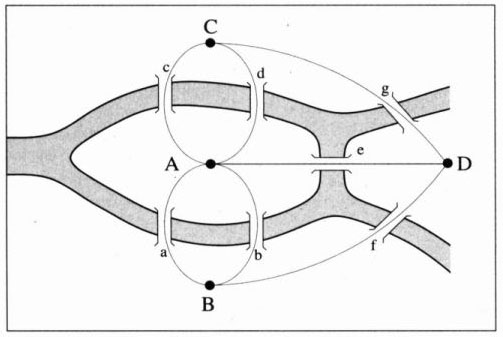
\includegraphics[width=0.75\textwidth]{img/Bridges.jpg}
\caption{Démonstration du problème des septs ponts de Königsberg}
\end{figure}

\subsection{Définitions}
Avant de parler des avantages des graphes, il est important de connaitre la léxique autours de le théorie des graphes \cite{WikiGraphes}.
\begin{description}
\item[Graphe]: un graphe est composé de sommets, et d'arêtes reliant certains de ces sommets.
Un graphe G est défini de manière formelle par un couple (S,A) où :
\begin{itemize}
	\item S est un ensemble fini d'éléments. Chacun de ces éléments est appelé sommet du graphe.
	\item A est un sous-ensemble (éventuellement nul) de SxS. Chacun de ces éléments de A est appelé arête.
\end{itemize}
\item[Arête :] c'est un connexion entre deux sommets A et B. Dans le cas où ce lien est orienté, le terme \textbf{arc} est généralement utilisé.

\item[Poids:] chaque arc/arrête est associé à un poids ou une étiquette qui le décrit. Par exemple, dans un réseau social il peut définir la nature de la relation (ami, famille, collègue) et dans un réseau routier la longueur d'une rue. Parfois le terme \textbf{coût} est utilisé pour décrire le poids.

\item[Successeurs et prédécesseurs:] dans un arc (x, y) d'un graphe, le sommet \emph{y} est appelé \textbf{successeur} de \emph{x} et \emph{x} est dit \textbf{prédécesseur} de \emph{y}.\newline
les sommets \emph{x} et \emph{y} sont des sommets voisins (ou adjacents).

\item[Graphe connexe] : un graphe est connexe si on peut atteindre n'importe quel sommet à partir d'un sommet quelconque en parcourant différentes arêtes/arcs.

\item[Graphe directionnel] : aussi appelé graphe orienté, digraphe ou un réseau dirigé, c'est un graphe où tous les sommets sont reliés par des arcs.
Un graphe où les sommets sont reliés par des arêtes est appelé un graphe non-orienté

\item[Chemin] : un chemin est une suite finie et consécutive de sommets et d'arcs, ou d'arcs uniquement, débutant et finissant par un sommet source et un sommet destination, tel que chaque arc sortant d'un sommet est incident (entrant) au sommet suivant dans cette séquence.
La figure \ref{fig:chemin} donne un exemple d'un chemin orienté.
\begin{figure}[h]
	\centering
	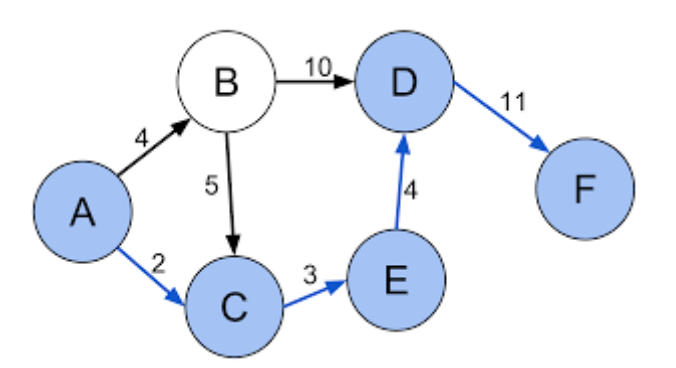
\includegraphics[width=0.55\textwidth]{img/cheminGraphe.png}
	\caption{Exemple de chemin orienté}
	\label{fig:chemin}
\end{figure}
\end{description}

	
	
\section{Avantages d'utilisation d'un graphe}
\subsection{Domaines d'utilisation des graphes}
Un graphe sert avant tout à manipuler des concepts, et à établir un lien entre ces concepts. N'importe quel problème comportant des objets avec des relations entre ces objets peut être modélisé par un graphe.
Les graphes sont donc des outils très puissants et largement répandus qui se prêtent bien à la résolution de nombreux problèmes. Voici quelques-uns \cite{domainesGraphe}:

\begin{description}


\item[Recherche de chemin (PathFinding)]
Un cas très fréquent. Chaque nœud représente une position et chaque arête est un chemin entre deux positions, ou en remplaçant les nœuds par des adresses et les arêtes par des routes, on obtient le graphe utilisé par les GPS ou les outils de cartographie tel que Google Map.
La recherche de chemins est aussi utilisée en biologie, communications (réseaux de télécommunications)...etc.
Il est courant de chercher le chemin le plus court entre deux positions dans la plupart de ces domaines, nous nous intéressons particulièrement à ce cas d'utilisation, que nous discuterons en détail dans la section suivante.


\item[L'ordonnancement de tâches:]
On peut représenter chacune des tâches à effectuer par un nœud, et les dépendances entre chacune de ces tâches par des arcs.
On cite l'exemple de l'ordonnancement des projets, les graphes permettent de planifier les différentes tâches d'un projet, détecter les tâches pouvant être effectuées simultanément et estimer la durée totale du projet.

\item[Les systèmes de recommandation:]
C'est une forme spécifique de filtrage de l'information qui a pour but de présenter à un utilisateur des éléments qui sont susceptibles de l'intéresser, en se basant sur ses préférences et son comportement.
Les moteurs de recommandation font usage des graphes pour représenter des individus ou objets et leurs différents liens. Cet outil est très utilisé en sciences sociales, par exemple le graphe social de Facebook qui représente les associations entre des personnes ou le réseau LinkedIn qui est un graphe de relations entre des professionnels...etc.

Le but est de pouvoir identifier les communautés formées, les centres d'intérêts communs, en suggérant à l'utilisateur les choses qu'il est susceptible d'aimer, les personnes qu'il connaît peut-être, et avant tout (et surtout) pour créer des publicités ciblées adaptées à chacun.

\end{description}

\section{Recherche de Chemin:}

\subsection{Définition:}
La recherche du plus court chemin est la capacité pour un système de déduire le chemin approprié autour des obstacles pour atteindre un point de destination tout en évitant les obstacles et en parcourant la distance la plus petite possible.
Le choix de la méthode de l'analyse et sa complexité peuvent augmenter à mesure que d'autres circonstances doivent être analysées, en prenant en compte différentes contraintes :

\begin{itemize}
	\item \textbf{Poids:} certains algorithmes n'acceptent que des arcs dont le poids est positif.
	\item \textbf{Type d'algorithme:} il existe des algorithmes qui calculent le plus court chemin de nœud à nœud, entre toutes les paires de nœuds ou encore d'un nœud vers tous les autres.
	\item \textbf{Prise en compte d'informations externes:} l'utilisation d'une connaissance externe à la structure du graphe peut parfois accélérer la recherche.
\end{itemize}

\subsection{Domaines d'utilisation :}
Le problème du plus court chemin est parmi les problèmes les plus étudiés de la théorie des graphes, on le retrouve dans beaucoup de domaines :
\begin{itemize}
\item\textbf{Optimisation des réseaux:} réseaux routiers, de télécommunications, de distribution.
\item\textbf{Réseaux informatiques et protocoles de routage: } les protocoles de routages permettant de trouver les meilleurs chemins pour passer les paquets réseaux utilisent ces algorithmes, tel que le protocole OSPF (Open Shortest Path First).
\item\textbf{Biologie:} il est utilisé pour étudier la propagation d'une maladie infectieuse, par exemple.
\item\textbf{Cartographie:} pour mesurer le chemin le plus court entre deux lieux ou villes.
\end{itemize}

\subsection{Les algorithmes de recherche de chemin}
Les algorithmes de calcul d'itinéraires origine-destination(s) sont des algorithmes qui permettent de calculer le plus court chemin d'un sommet source vers tous les autres sommets avec une complexité polynomiale.\newline
 On les répartit classiquement en deux familles : 
\begin{itemize}
	\item \textbf{A fixation d'étiquette} (Label setting algorithms): Ce type d'algorithme choisissent à chaque itération un sommet x, et calculent sa valeur définitive V[x]. Cette valeur V[x], appelée étiquette, sert à définir la valeur du plus court chemin vers le sommet x.
	L'avantage principal de ces algorithmes est qu'il est possible d'arrêter la recherche de chemin dès atteinte du nœud destination puisque son étiquette sera fixée définitivement.
	L'algorithme à correction d'étiquette le plus célèbre est l'algorithme de \textbf{Djikstra}\cite{Djikstra}.
	
	\item \textbf{A correction d'étiquette} (Label correcting algorithms): Ces algorithmes peuvent affiner et corriger les étiquettes de chaque sommet jusqu'à la dernière itération.
	Ils ne sont pas forcément moins performants que les algorithmes à fixation d'étiquette, et ont une utilisation plus générale, lors de présence de poids négatives dans le graphe où l'algorithme de Djikstra, par exemple, n'est pas utilisable.\newline
	Un exemple bien connu est l'algorithme de \textbf{Bellman-Ford}.
\end{itemize}

Malgré leur complexité polynomiale, ces algorithmes peuvent engendrer des temps de calculs importants pour des graphes de grande taille, ce qui a suscité le développement des techniques d'accélération (visant souvent l'optimalité plutôt qu'un meilleur chemin) comme l'algorithme A* qui est le plus célèbre, le parcours en largeur/profondeur, le parcours bidirectionnel, ainsi que les méthodes de pré-traitement (pré-calculer les meilleurs chemins dans tout les nœuds par exemple).

Dans notre cas, et vu que le graphe de la première version est statique (ne changera pas après avoir calculé le chemin), le choix le plus pertinent serait l'\textbf{algorithme A*} \cite{Astar}.
Cependant, ce dernier nécessite une fonction heuristique\FancyFootNote{Heuristique: une méthode de calcul qui fournit rapidement une solution réalisable, pas nécessairement optimale ou exacte, pour un problème d'optimisation difficile.} pour estimer le meilleur nœud suivant, ce qui sera difficile à concevoir sans une bonne connaissance de notre problème et dans les limites du temps de ce projet.
De ce fait, nous avons opté pour une approche plus simple utilisant l'algorithme BFS qui est simple à implémenter et à adapter à nos besoins, pour ainsi avoir rapidement une version minimale de l'application, cet algorithme sera présenté dans la section suivante.\newline
Nous avons pris en compte la possibilité de changer l'algorithme de recherche dans de futures version de l'application, en prenant une structure plus flexible qui sera expliquée dans le chapitre suivant.

\subsection{L'algorithme BFS (Breadth-First-Search)}

\begin{enumerate}
	\item \textbf{Présentation}: BFS\cite{refBFS} est un algorithme de parcours ou de recherche dans un arbre ou graphe, il commence d'un nœud source (ou la racine de l'arbre) et explore ses nœuds successeurs d'abord, 

Cet algorithme est très similaire au parcours par largeur d'un arbre, sauf qu'un graphe peut avoir des cycles, donc pour éviter de recalculer le même nœud deux fois, il garde une liste de nœuds visités.

	\item \textbf{Complexité:} la complexité temporelle de l'algorithme est de O(V+E), où V est le nombre de sommets et E le nombre d'arcs.
	
	\item \textbf{Étapes de l'algorithme:}
		L'algorithme effectue un parcours en largeur sur le graphe, en d'autres mot un parcours par niveau, il traite tous les nœuds voisins du nœud de départ avant de passer aux nœuds voisins des nœuds visités.
\begin{figure}
	\center
	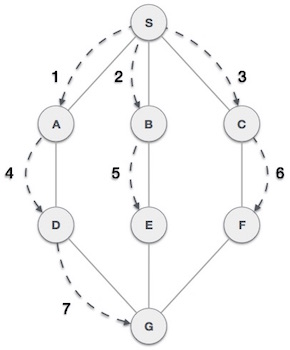
\includegraphics[scale=0.6]{img/BFS.jpg}
	\caption{Déroulement d'un parcours BFS.}
\end{figure}		
L'algorithme utilise une file pour mémoriser les nœuds suivants à visiter, les étapes de l'algorithme se résument en les règles suivantes:
	\begin{enumerate}
		\item Visiter le nœud suivant non visité du nœud courant, le marquer comme visité, traiter le nœud et l'insérer dans la file.
		\item Si aucun autre nœud voisin n'est trouvé, retirer le premier nœud de la file.
		\item Répéter les étapes (a) et (b) jusqu'à ce que la file soit vide.
	\end{enumerate}
	Le BFS traverse donc seulement les nœuds qui peuvent être atteints depuis le nœud de départ.
\end{enumerate}

\section{Collecte de données}
Afin de mieux tester notre application, nous avons tenté de collecter un maximum de données réelles, à commencer par contacter l'Entreprise de Transport d'Oran, puis ensuite traiter ces informations et ajouter d'autres que nous avons collectés par nous-mêmes.
Le résultat de cette collecte est comme suit :

\subsection{ETO (Entreprise de Transport d'Oran)}

%what they did gave u
Nous avons été bien accueillis par l'un des responsables de l'ETO que nous remercions de nous avoir bien expliqué le fonctionnement des lignes de notre région ainsi que d'avoir fourni plusieurs informations utiles, tel que:
\begin{itemize}
	\item La liste des lignes et leur longueur totale.
	\item Les différents horaires de travail (été/hiver/fin de semaine...etc).
	\item La fréquence des bus et les différentes contraintes spécifiques à notre région, comme le manque de calendrier d'horaires qui décrivent le temps de passage de chaque bus.
	\item Le nombre de bus desservant chaque ligne.
	\item Le nom de chaque station.
\end{itemize}

% but that wasnt enough
En plus du catalogue que nous avons reçu, leurs informations nous ont permis de bien tracer les spécifications et les particularités de ces lignes.
Cependant, ces informations n'ont pas été suffisantes pour notre travail, en effet:
	\begin{itemize}
	\item Nous avions besoin de noms plus significatifs pour chaque station, car les noms fournis étaient des noms communs connues par les habitants seulement.
	\item Le catalogue ne contenant pas les adresses exacte ou les coordonnées de chaque station.
	\item Pas d'informations sur la distance entre chaque station.
	\end{itemize}
	
%thx again for trying
Nous remercions encore l'ETO pour leur assistance, néanmoins ces données doivent être traitées davantage, réorganisées et complétées avant qu'elles puissent être intégrées dans notre application.

\begin{figure}
	\center
	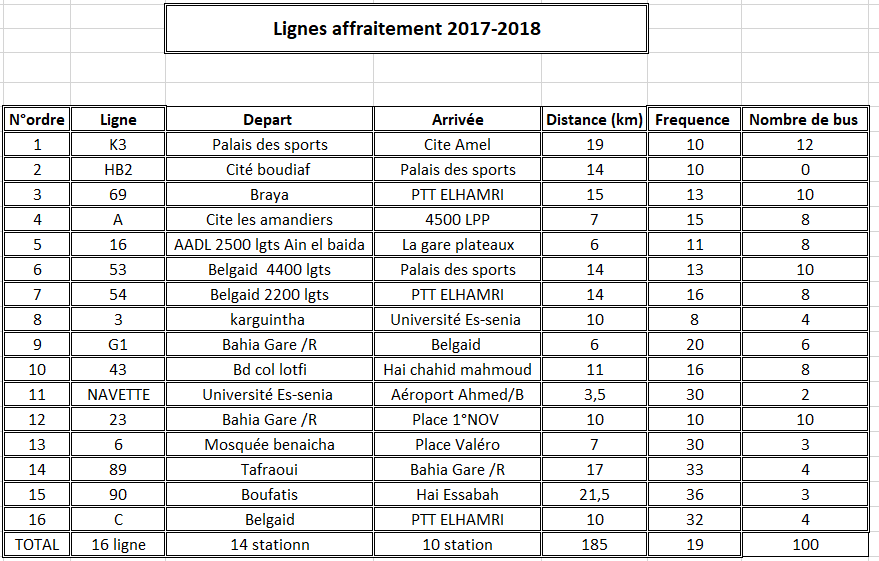
\includegraphics[scale=0.7]{img/LignesETO.png}
	\caption{Échantillon de données reçues par l'ETO.}
\end{figure}

\subsection{Données supplémentaire}
	\begin{itemize}
		\item Malgré l'absence de données officielles, nous avons réussi à trouver sur le net différentes sources supplémentaires pouvant nous aider pour compléter nos données : notamment des listes de différents lieux de la ville d'Oran contenant des noms complets et des adresses permettant de compléter les données de l'ETO.
		\item Le site officiel de la Setram (Société d'Exploitation des Tramways) a été suffisant pour récupérer toutes les données concernant la ligne du Tramway, ses horaires et même les temps d'attente pour chaque arrêt.
		\item Pour assurer l'intégrité des données et leurs mise à jour constantes, une des solutions proposées est d'ajouter une fonctionnalité permettant à des utilisateurs ou à une autorité de signaler un changement de lignes, une estimation de temps trop imprécise ou suggérer des chemins que l'application n'a pas calculé, ceci permettra de faire fonctionner et évoluer cette application à l'aide de \emph{crowdsourcing}\FancyFootNote{crowdsourcing: ou production participative, c'est l'utilisation de connaissance d'un grand nombre de personnes comme une communauté d'internautes ou des utilisateurs d'un produit, pour réaliser une tâche traditionnellement faite par des employés.} seulement.
	\end{itemize}

\subsection{Traitement de données}
Les données obtenues de l'ETO et de l'Internet ont permis de rassembler les informations suivantes :
\begin{itemize}
	\item Différentes informations sur le fonctionnement de lignes.
	\item Liste des lignes de bus publiques et les stations desservies, les noms des stations étant toujours pas claires et sans adresses.
	\item Longueur totale de chaque ligne, fréquence et nombre de bus de chaque ligne.\newline 
\end{itemize}

Depuis ces informations nous avons déduit d'autres informations utiles, notamment :

\begin{itemize}
	\item \textbf{Temps d'attente : } Les bus n'ayant pas de calendrier précis, nous avons utilisé la distance totale, fréquence et nombre de bus pour déduire approximativement le temps d'attente dans chaque arrêt entre deux bus.
	\item \textbf{Coordonnées GPS :} Afin d'afficher les stations sur une carte, les coordonnées GPS, ou au moins des adresses précises permettant de générer les coordonnées avec un outil de cartographie, sont nécessaires. Cependant, les données que nous avons ne sont pas suffisantes.
	L'application administrateur de ce projet nous a néanmoins permis de marquer les stations sur une carte et enregistrer les informations nécessaires automatiquement. L'aperçu de cette interface est donné dans la section \ref{ref:Implementation}.

\end{itemize}

	
\section{Construction du graphe}
Après avoir présenté quelques généralités sur graphe, et détaillé les données que nous avons collecté, nous passons aux différents détails sur comment est construit notre graphe et comment le stocker.
\subsection{Différentes approches pour stocker le graphe}
\begin{itemize}
	\item \textbf{Outils Open Source (OpenTripPlanner)} : 
	      Il existe plusieurs outils qui proposent ce service, en particulier OpenTripPlanner\cite{OpenTripPlanner} : un projet Open Source qui permet de créer un réseau routier à partir de données GTFS \FancyFootNote{GTFS (General Transit Feed Specification ou spécification générale pour les flux relatifs aux transports en commun) : est un format informatique standardisé pour communiquer des horaires de transports en commun et les informations géographiques associées.}, ces données seront ensuite intégrées avec OpenStreetMap et stockées sur le serveur, qui exposera une API REST pour questionner le serveur : recherche de Chemin, possibilité d'intégrer les horaires, ...etc.
	      		
	      Vu la nature un peu particulière du réseau d'Oran, et la non-disponibilité des données (Données officielles des lignes et données (adresses) sur OpenStreetMap), cette solution ne sera pas envisagée. 
	      Cependant, l'application prendra une architecture flexible permettant d'intégrer, au futur, de tels outils rapidement si une solution est possible.
	\item \textbf{Représentation indépendante de chaque ligne en tables SQL}
	      Une des approches considérées était de représenter chaque ligne indépendamment, l'algorithme du service aura à chercher des points de liaison entre ces lignes.
	      L'avantage principal de cette approche est la facilité de manipulation de ces données de lignes, en ajoutant/supprimant des lignes sans conflit.
	      Cette approche présente par contre un inconvénient majeur au niveau des performances, vu que l'utilisation d'un algorithme de PathFinding requiert l'utilisation de plusieurs tables (lignes) à chaque requête.
	      
	\item \textbf{Utiliser une base de données orientée graphe}: nous avons finalement choisi d'utiliser une base de données orientée graphe qui permet de stocker en permanence le graphe, mais aussi de fournir plusieurs opérations pour créer des nœuds et des relations, les modifier et les parcourir pour rechercher des chemins ou effectuer certains calculs.
	
Comparé au stockage par tables SQL, cette approche offre un accès plus rapide et simple en parcourant un graphe déjà construit tout en tirant les meilleures performances des différents algorithmes de recherche de chemins.

	Nous avons, cependant, noté certaines difficultés suivant cette représentation, notamment dans la modification ou suppression de lignes où le changement ou la suppression d'une seule station peut affecter plusieurs autres lignes.\newline
	Ainsi, comme l'ajout d'une station au milieu d'une ligne impliquera la suppression de plusieurs arcs, nous avons décidé, comme première solution, de restreindre les modifications et suppressions de nœuds aux stations qui ne sont reliées à aucune ligne, et pour les lignes, de supprimer toute la ligne et reconstruire les arcs à chaque modification.
	     
\end{itemize}
\subsection{Représentation choisie du graphe}
La figure \ref{fig:structGraph} présente la structure utilisée pour représenter toutes nos données dans le graphe:
\begin{itemize}
	\item Chaque nœud avec l'étiquette \emph{:Station} représenterait une station de transport quelconque.
	\item Chaque arc entre stations représente le passage d'un transport public entre ces deux stations, ces arcs sont étiquetés par le type du transport (Bus, Tramway,..etc.), chaque type contient les différentes données de chaque transport comme le nom du Bus.
\end{itemize}

\begin{figure}[h!]
	\center
	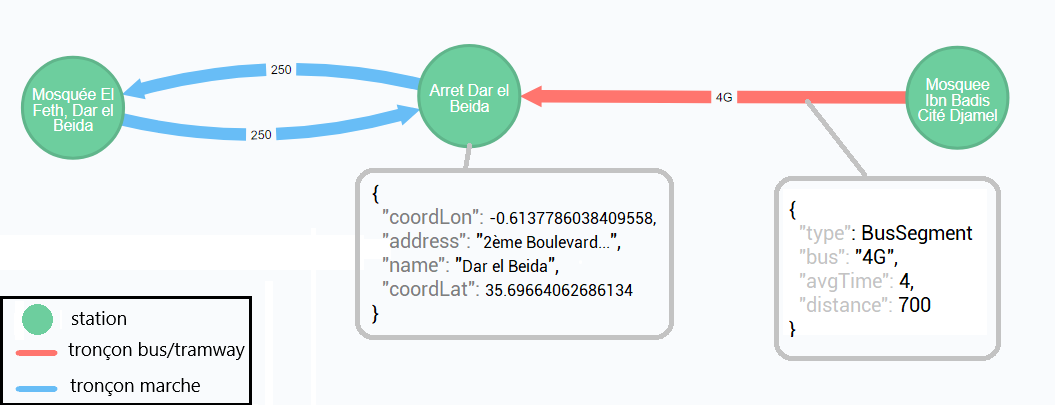
\includegraphics[width=\textwidth]{img/structureGraphe.png}
	\caption{Représentation en graphe du réseau routier}
	\label{fig:structGraph}
\end{figure}

\begin{figure}[h!]
	\center
	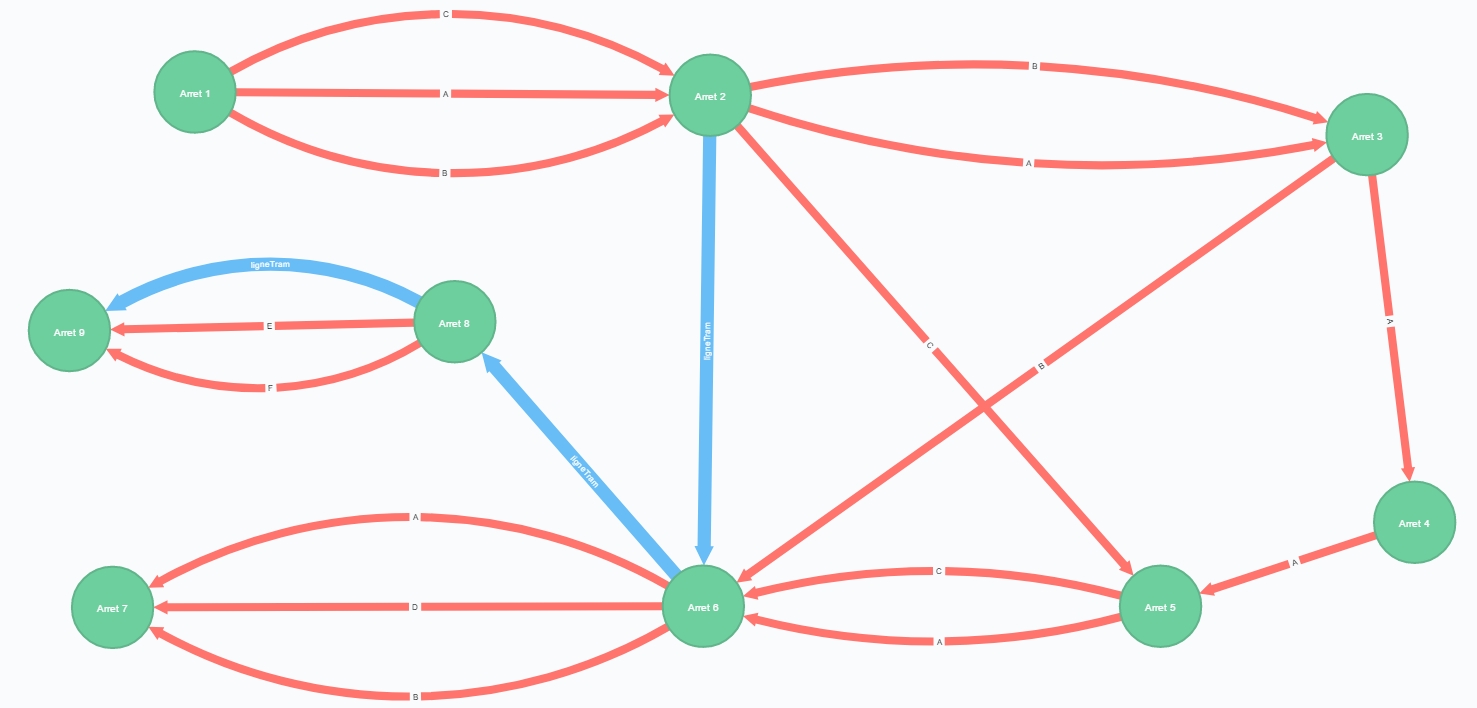
\includegraphics[width=1.1\textwidth]{img/GrapheNeo4j.png}
	\caption{Aperçu d'un graphe de transport}
\end{figure}

\textbf{Arcs de bus: } Chaque arc contient uniquement l'identifiant du Bus qui le concerne, les autres informations de chaque bus (temps d'arrêt, prix...etc.) peuvent être représentés séparément comme d'autres nœuds étiquetés dans le graphe ou stockés ailleurs dans une base de données différente. \newline
Nous avons choisi de ne garder que les données les plus importantes dans cette première version, nous pouvons ajouter d'autres propriétés et informations dans le graphe au fur et à mesure que l'application évolue.

%
%	\begin{itemize}
%		 \item Arcs étiquetés par le type du transport ( BusSegment, TramSegment, WalkSegment. ..) 
%		 \item Représenter chaque bus séparément ( pour faciliter la recherche et filtre ) 
%		 \item Nœuds (Stations) ont les attributs suivants : 
%		 \begin{itemize}
%		 	\item Nom.
%		 	\item Adresse.
%		 	\item Tableau de coordonnées (pour chaque direction) avec indicateur de direction.
%		 \end{itemize}
%		 \item Arcs ont les attributs suivants :
%		 \begin{itemize}
%		 		\item Dist : distance entre les deux stations
%		 		\item Time: temps moyen pour passer de la première station à la deuxieme
%		 		\item Bus : ( pour les arcs de type Bus ) nom/id du bus.
%		 		** remarque : infos du bus ( temps d'arrêt, prix ..etc) sont stockés sépareraient.
%		 \end{itemize}
%	\end{itemize}

\subsection{Cas de la marche}
Afin de pouvoir intégrer la marche dans la recherche de chemin, il est nécessaire de pouvoir détecter les arrêts les plus proches de chaque arrêt pendant le traitement, et essayer de considérer les arrêts les plus proches de chaque nœud visité.\newline 
Cette solution s'avère difficile à appliquer dans la version actuelle du projet, nous avons donc choisi de représenter la possibilité de marcher avec un arc similaire aux arcs de transports.\newline
Ces arcs sont automatiquement ajoutés à la création de chaque ligne en calculant toutes les distances entre le début et fin de la ligne ajoutée avec le début et fin de chaque autre ligne, et ajouter un arc dans les deux sens si la distance est inférieur à 1Km (valeur arbitraire).
Un exemple de cet arc est donné dans la figure \ref{fig:structGraph}.

Cette approche permet d'intégrer la marche de façon minimale sans affecter les performances et sans avoir à calculer des distances pendant la recherche du chemin.
Il sera possible d'améliorer cette fonctionnalité après avoir implémenté la recherche des plus proches stations directement dans le graphe à partir d'un point donné, sans avoir à comparer toutes les stations (voir chapitre des perspectives).

\section{Conclusion}
Nous avons, dans ce chapitre, présenté les différentes généralités sur les graphes et données collectés ainsi que comment est construit notre graphe pour ce projet.
Malgré les différentes contraintes (complexité du problème, manque de données, spécificités des lignes d'Oran), la représentation choisie pour cette première version reste suffisante et facilement extensible pour de futures améliorations.
\newpage

%Chapitre 4
\chapter{Développement}
Après avoir détaillé la représentation des données de ce projet, nous étudierons dans ce chapitre les différentes technologies utilisées dans l'implémentation ainsi que l'architecture utilisée. Nous détaillerons ensuite les formats et modèles de nos données. Enfin, nous donnerons un aperçu des applications front-end.
\section{Technologies utilisées}
\subsection{NodeJs}
Aux alentours de 2010 Google a commencé à rendre JavaScript et son moteur d'exécution V8 plus rapides. Des outils comme Nodejs sont ensuite apparus\cite{NodeJs}.\newline
Node.js est un environnement d'exécution \textbf{JavaScript} construit sur le moteur \emph{V8} de Google Chrome. Il utilise un modèle basé sur l'événementiel (\textbf{event-driven}) et des entrées/sorties non bloquantes, ce qui le rend léger et efficace.
Il présente plusieurs avantages, notamment :
\begin{itemize}
	\item NodeJs et son écosystème permettent de travailler avec JavaScript à la fois sur le frontend et le backend.
	\item L'approche non bloquante de NodeJs lui permet d'effectuer des entrées/sorties (I/O) de manière asynchrone. La programmation asynchrone est idéal pour une exécution plus rapide de programmes.
	\item Contrairement aux langages serveur célèbres tel que PHP, ASP.NET, Ruby ou Java, NodeJs s'exécute en \emph{monothread}, en d'autres termes les processus de chaque requête sont traités dans un seul fil d'exécution, ce qui est très efficace en termes de mémoire.
	\item NodeJs rassemble une grande communauté très active, ce qui offre un grand nombre de librairies et de support en travaillant avec NodeJs.\newline
\end{itemize}

\textbf{ExpressJs :} un framework\FancyFootNote{Framework : C'est une sorte d'infrastructure de développement, il désigne un ensemble cohérent de composants logiciels structurels qui sert à créer les fondations ainsi que les grandes lignes de tout ou d'une partie d'un logiciel ou application.} d'application minimaliste et très flexible qui propose un ensemble de fonctionnalités stables pour les applications web, en l'occurrence l'implémentation des APIs (Express.Router). Au moment d'écrire ce rapport, c'est l'outil le plus connu et le plus utilisé avec NodeJs.

NodeJs est donc un choix idéal pour développer des APIs REST minimales et flexibles tout en gardant des performances élevées pendant le traitement de requêtes.\newline
En dernier, bien que NodeJs ne soit pas adapté pour des applications aux calculs intensifs, il ne sera pas un inconvénient du fait que les calculs sur le graphe seront effectués principalement dans le SGBD.
\subsection{MongoDB}
	MongoDB \cite{MongoDB} est un système de base de données NoSQL. Il est orienté documents qui est une évolution des simples bases de données clé-valeur. Un document peut être une valeur atomique, paire clé-valeur, un tableau de valeurs ou une compositions de ces derniers.

Son nom vient de Humongous qui veut dire énorme ou immense. Il est capable de gérer de très grandes quantités de données avec une grande facilité d'extension, ses principaux avantages sont:

\begin{itemize}
	\item Stockage flexible de données sous forme de documents semi-structurés (similaires au JSON), les attributs peuvent varier de document à document et la structure peut changer au fil du temps.
	\item Facilité de manipulation depuis l'application: MongoDB transforme les documents en objets qui peuvent être manipulés avec le langage de programmation utilisé.
	\item Existence de méthodes puissantes pour accéder et analyser les données.
\end{itemize}

En résumé, MongoDB est un SGBD très flexible et simple à utiliser, nous stockerons les informations supplémentaires de notre application en utilisant ce système, tel que les Bus, horaires,...etc.

\subsection{Neo4j}
Apparu en l'année 2000 et appartient à la société Neo Technology, Neo4j \cite{Neo4j} est un système de gestion de bases de données (SGBD) orienté graphe. Son approche est fondée sur la théorie des graphes. Les données sont stockées de manière assez libre (sans modèle prédéfini) dans des nœuds reliés entre eux par des relations.

Ses principaux avantages sont :
\begin{itemize}
	\item Neo4j utilise un stockage natif du graphe, avec un principe appelé \textbf{index-free adjacency}, ceci permet de stocker des nœuds directement avec ses relations et nœuds adjacents sans avoir à utiliser des indexes pour consulter ses relations.\newline
	Le stockage natif offre de très grandes performances de lecture/écriture indépendamment de la taille du graphe (le temps d'accès à chaque noeud est constant).
	\item Neo4j est open-source, et a la plus grande communauté dans les bases de données orientées graphe, qui contribuent constamment à son écosystème, ce qui donne un très grand nombre de ressources et de support ainsi qu'une grande liste de pilotes et librairies dans tous les langages courants.
	\item Neo4j se présente comme une solution dans un très grand nombre de cas d'utilisations, par exemple: Réseaux sociaux, détection de fraude, Réseaux et opérations IT...etc.
	\item Facile à apprendre et à utiliser: Neo4j dispose d'une interface graphique très moderne et riche, et utilise son propre langage d'interrogation Cypher.\newline
\end{itemize}

Neo4j étant le SGBD le plus dominant dans le domaine des SGBD orientés graphe, et offrant une grande performance et flexibilité qui satisfait tous les besoins de ce projet. Nous n'avons pas eu besoin de considérer les autres systèmes.

\textbf{Cypher: } c'est un langage de requête déclaratif sur Neo4j. Il permet de décrire la forme du résultat et les contraintes souhaitées à ajouter en optimisant le plan d'exécution pour récupérer les résultats.\newline

Il utilise une syntaxe déclarative similaire au SQL, avec de l'ASCII Art (des figures et signes utilisant des lettres et caractères spéciaux) pour décrire les nœuds et les relations, rendant les requêtes faciles à lire et comprendre. Un exemple est donné dans la figue \ref{fig:cypher}.

\begin{figure}
	\center
	\includegraphics[width=0.8\textwidth]{img/cypher.png}
	\caption{Exemple de requête Cypher.}
	\label{fig:cypher}
\end{figure}

\subsection{VueJs}
VueJs\cite{VueJs} est un framework évolutif pour construire des interfaces utilisateur. Il a été conçu et pensé pour pouvoir être adopté de manière incrémentale. Le cœur de la bibliothèque est concentré uniquement sur la partie vue, le reste (Routage, gestion d'état...) étant fourni dans des bibliothèques complémentaires, et il est simple de l'intégrer avec d'autres bibliothèques ou projets existants. 
Il est tout à fait capable de faire tourner des applications web monopages (Single Page Applications) très complexes lorsqu'il est combiné avec d'autres outils modernes et ses bibliothèques complémentaires.\newline
Ses principaux avantages sont : 
\begin{itemize}
	\item Très petit de taille et facile à apprendre: possible de commencer le développement avec VueJs rapidement sans avoir à connaitre toutes les fonctionnalités avancées dès le départ.
	\item Très bien documenté avec une communauté active.
	\item Flexible et offre de très bonne performances, c'est un des framework les plus rapides en ce moment.
\end{itemize}

Il est très difficile de comparer les framework front-end, chacune a ses points forts et toutes peuvent accomplir le même résultat. Nous avons opté pour VueJs à raison de sa grande flexibilité et la facilité de commencer avec, qui nous a permis de tester rapidement plusieurs outils et fonctionnalités avant d'atteindre le résultat donné dans la section \ref{ref:Implementation}.

\section{Structure de l'application}
\subsection{L'architecture MVC (Model-View-Controller)}
L'architecture MVC est un modèle d'architecture qui sépare une application en 3 composants logiques: \textbf{Model}, \textbf{View}, \textbf{Controller}.
Chaque composant est construit pour gérer un aspect spécifique de l'application, on peut résumer le rôle de chacun comme suit :
\begin{enumerate}
	\item \textbf{Models: } ces composants correspondent à tout ce qui est relié aux données, un model peut représenter une classe d'objets ou une structure de données échangée entre Views et Controllers, ainsi que la logique manipulant ces données telle que des calculs de moyennes ou les différentes opérations d'ajout, modification et suppression dans une base de données.
	\item \textbf{Views:} les views sont utilisés pour l'interface utilisateur (UI) de l'application, ceci inclut les composants d'interface (textes, boutons, formulaires...etc.), ainsi que certaines logiques de mise en forme et affichage des données.
	\item \textbf{Controller: } le Controller joue le rôle d'une interface entre le Model et les Views afin de traiter les requêtes venant du View (par exemple un clique de bouton), manipuler les données du Model et enfin les rendre au View pour qu'elles soient présentées. il contient généralement la logique des actions effectuées par l'utilisateur.
\end{enumerate}
	
MVC est une des architectures les plus utilisées pour créer des projets évolutifs et extensibles \cite{refMVC}.
%Il existe plusieurs variantes du MVC et d'autres architectures similaires tel que le MVVM (Model-View-ViewModel) et le MVP (Model-View-Presenter).

\subsection{Composants de l'application}
L'application suit une architecture MVC décomposée comme suit :
\begin{sidewaysfigure}
	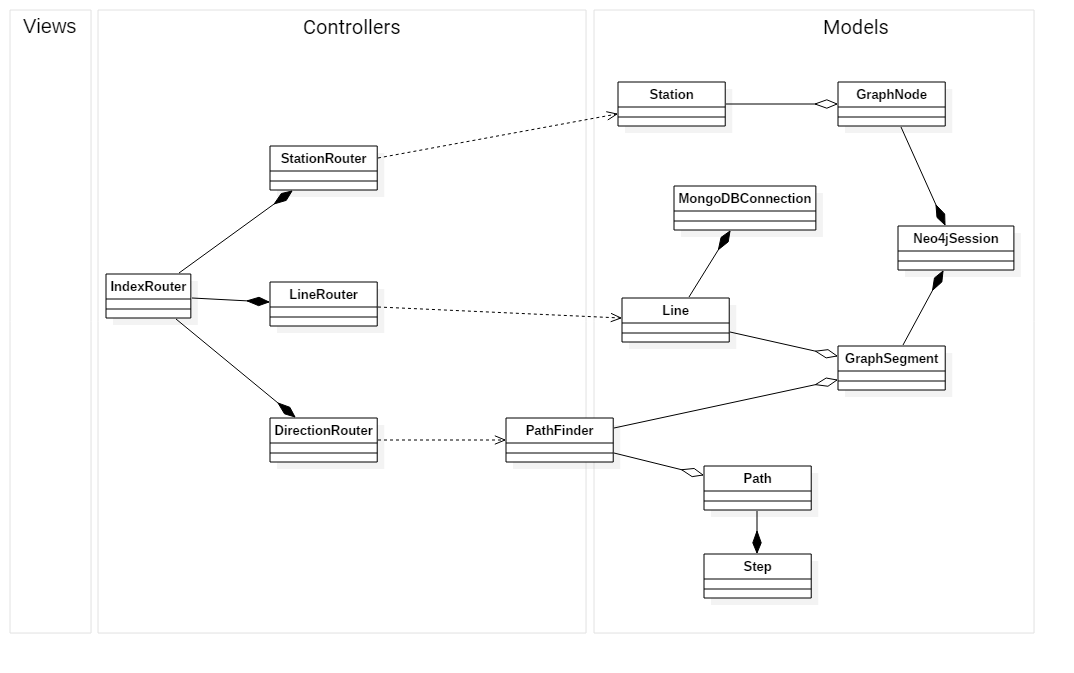
\includegraphics[width=\textwidth]{img/ClassDiagram.png}
	\caption{Vue d'ensemble des composants de l'application}
	\label{fig:classDiagram}
\end{sidewaysfigure}	
\begin{enumerate}
	\item \textbf{Models:}
	      \begin{itemize}
	      	\item \textbf{Station} : représente une station avec son nom, adresse et coordonnées.
	      	\item \textbf{Line} : représente une ligne de transport, le format complet est décrit dans la partie \ref{ref:resources}.
	      	      \begin{itemize}
	      	      	\item \textbf{Bus} : représente un Bus ainsi que les différents facteurs estimés (temps d'attente moyen, fréquence ...etc.).
	      	      \end{itemize}
	      	\item \textbf{Path} : représente une suggestion de chemin, contenant les informations globales tel que le prix et temps total du chemin, ainsi qu'une liste d'objets Step.
	      	      \begin{itemize}
	      	      	\item \textbf{Step} : représente une étape d'un itinéraire utilisant le même moyen de transport, comporte la station de départ et d'arrivée, les stations intermédiaires et les informations sur le temps, coût et distance à parcourir.
	      	      \end{itemize}
	      	      le format de cet objet est détaillé dans la section \ref{ref:formatReponse}
	      	\item \textbf{Models du graphe} : 
	      	      afin d'avoir une application facilement extensible, nous avons séparé les Models relatifs au graphe des Models de l'application, ce qui permettra de modifier la représentation du graphe sans affecter l'application.
	      	      \begin{itemize}
	      	      	\item \textbf{GrapheNode} : représente un nœud, communique avec la base de données pour créer et manipuler les nœuds.
	      	      	\item \textbf{GrapheSegment} : représente un arc entre deux nœuds, communique avec la base de données pour créer plusieurs relations (lignes de transport) ou les supprimer.
	      	      \end{itemize}
	      \end{itemize}
	      	
	\item \textbf{Controller :} dans le cas de notre application, le controller est le \emph{router} de l'application, ce dernier permet de définir les différents points terminaux (endpoints) de l'application et les identifier par une URI, les détails de l'API sont décrits dans la section suivante.
	     	      	
	\item \textbf{Views :} les Views dans ce projet consistent en deux applications séparées : une application client pour demander le chemin et consulter les lignes, et une application administrateur pour insérer et modifier les lignes des différents transports.
	      
	      Ces deux applications sont des \emph{Single Page Applications} : une application dynamique qui tourne sur un navigateur web.
	      Nous ne détaillerons pas l'implémentation de ces applications, car ce n'est pas l'objectif principal de ce projet. Un aperçu du résultat final est donné dans la section \ref{ref:Implementation}.
\end{enumerate}
La relation entre ces composants est décrite dans la figure \ref{fig:classDiagram}.
	
	
\section{Implémentation de l'API}
\label{ref:API}
\subsection{Ressources exposées}
Notre API définit principalement 3 ressources:
\begin{enumerate}
	\item \textbf{Station:} Ressource qui représente les différentes stations du réseau, elle accepte 3 requêtes différentes de type GET  : 
	      \begin{itemize}
	      	\item \emph{\textbf{/api/station}}: retourne toutes les stations, peut être utilisée pour visualiser toutes les stations par un client ou d'autres utilisations générales, le nombre de stations retournées seront limités et contrôlés par deux paramètres \textbf{limit} et \textbf{offset} afin d'éviter de retourner un très grand nombre de stations en une seule requête.
	      	\item \emph{\textbf{/api/station/\{id\}}}: retourne une station par identifiant, le client n'ayant rarement besoin de l'identifiant, cette URI est généralement utilisée du coté administrateur.
	      	\item \emph{\textbf{/api/station?match=\{name\}}}: Un paramètre dans la ressource station permet de retourner toutes les stations dont le nom contient la valeur \emph{name}, peut être utilisé pour la recherche et auto-complétion lors du choix du chemin, par exemple.
	      \end{itemize}
	      	      			
	      Cette ressource accepte aussi des requêtes de type POST (création), PUT (mise à jour) et DELETE (suppression)  pour les client administrateurs (authentifiés).
	\item \textbf{Ligne:} \emph{\textbf{/api/line}} : Ressource qui représente les différentes lignes de transport entre stations, elle accepte des requêtes de type GET du coté client, aussi des requêtes POST, PUT et DELETE du coté administrateur pour gérer les lignes.
	\item \textbf{Direction:}  \emph{\textbf{/api/direction}} : Ressource représentant les chemins, elle accepte seulement des requêtes de type GET, les détails de ces requêtes et leurs réponses sont détaillés dans la section \ref{SectionPathFinding}
\end{enumerate}
\subsection{Description des formats des ressources}
Les ressources principales de notre API sont les stations (\textbf{station}) et les lignes (\textbf{line}), leur format est décrit dans la figure \ref{fig:formatResources}.
\label{ref:resources}

\begin{description}
	\item[Station:] Dans cette version, chaque station contient un identifiant unique, le nom et l'adresse ainsi les coordonnées GPS.
	\item[Line:] Une ligne est identifiée par un ID et un nom, elle contient un lien vers le bus servant cette ligne et une liste des stations de cette ligne contenant l'identifiant, la distance et le temps entre chaque station. Cette ressource  est utilisée principalement pour les requêtes d'ajout du coté administrateur.
\end{description}
% Format JSON 
\lstset{style=JSON}

\begin{figure}[h!]
	%-------------------------------------------------------------------
	\begin{subfigure}[b]{0.45\linewidth}
		\begin{lstlisting}[caption=Format JSON de Station]
{
	ID: 1,
	name: "string",
	address: "string",
	coords: 
	[
	  {
	  	  direction: "string",
  		  lat: 0.00,
   		  lon: 0.00
	  }
	]
}
		\end{lstlisting}
	\end{subfigure}\hfill%  
	%-------------------------------------------------------------------
	\begin{subfigure}[b]{0.45\linewidth}
		\begin{lstlisting}[caption=Format JSON de Line]
{
  "id": 0,
  "name": "string",
  "bus": {
    "name": "string",
    "link": "/api/bus/{id}",
  },
  "lineStations": [
    {
      "stationID": 0,
      "distFromPrev": 0,
      "timeFromPrev": 0
    }
  ]
}
		\end{lstlisting}
	\end{subfigure}\hfill%  
	%-------------------------------------------------------------------
	\caption{Description du format des ressources.}
	\label{fig:formatResources}
\end{figure}


\section{Recherche de chemin}
L'implémentation de l'application du côté serveur permet de calculer un ensemble de chemins optimaux entre deux stations identifiées par un identifiant.
\subsection{Déroulement d'une requête}
\begin{sidewaysfigure}[h!]
	\center
	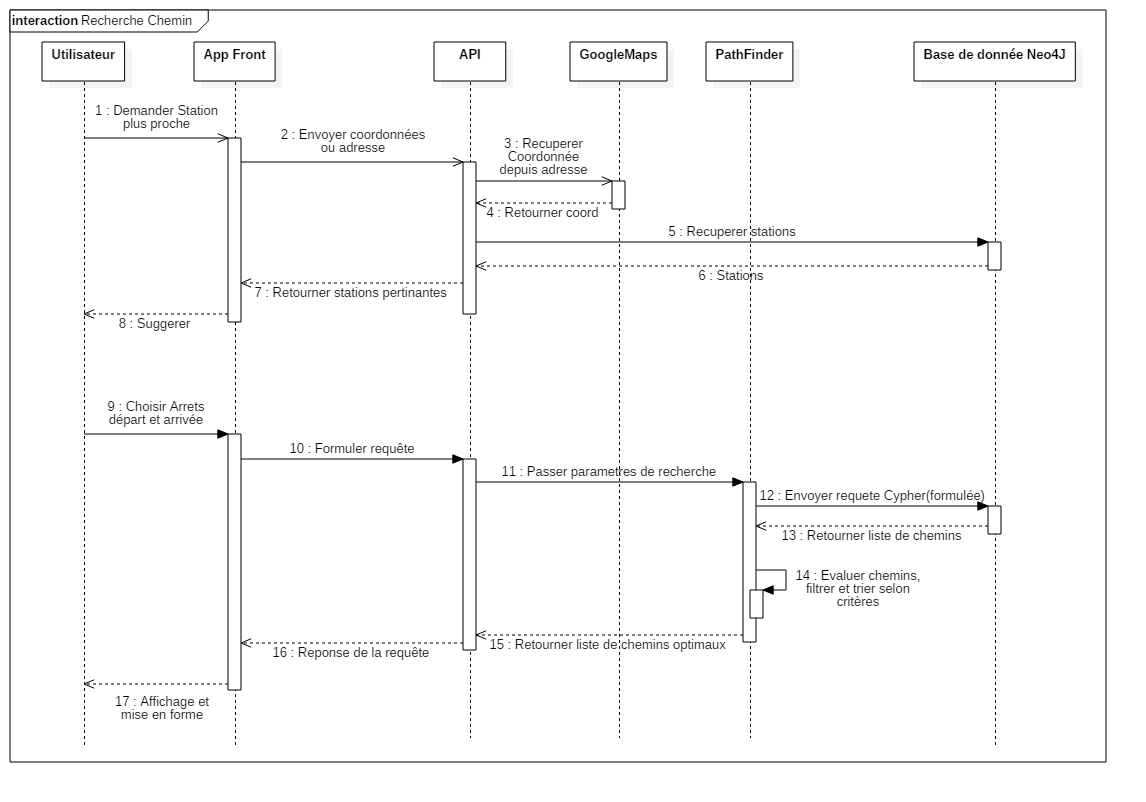
\includegraphics[width=\textwidth]{img/RechercheChemin.png}
	\caption{Diagramme de séquence pour la recherche de chemins.}
	\label{fig:diagSequence}
\end{sidewaysfigure}

Une requête de recherche d'itinéraire à commencer de la demande de l'utilisateur jusqu'à l'affichage de la réponse passe par plusieurs étapes. Le diagramme de séquence dans la figure \ref{fig:diagSequence} décrit les étapes suivantes :
\begin{enumerate}
	\item L'API reçoit la requête de chemin, vérifie les paramètres et met en forme les données, pour les passer au module qui calcule le chemin (PathFinder).
	\item Le module PathFinder formule la requête Cypher et l'envoi au serveur de la base de données Neo4j. Cette requête est décrite dans la partie \ref{section:cypher}.
	      Nous pouvons depuis cette requête filtrer les différents transports à inclure dans le chemin facilement, puisque chaque moyen de transport est désigné par ses propres arcs étiquetés dans le graphe.
	\item Neo4j retourne ainsi une liste de chemins optimaux, le module va ensuite évaluer chaque chemin :
	      \begin{itemize}
	      	\item Évaluer le temps et coût estimés de chaque chemin.
	      	\item Trier les chemins selon le critère de la requête, en cas d'égalité considérer les autres critères.
	      	\item Structurer chaque chemin en Objets Path, détaillé dans la section suivante.
	      	\item Minimiser le chemin en regroupant les étapes intermédiaires (tel que deux arrêts utilisant le même Bus).
	      \end{itemize}
	\item Retourner l'objet à l'API qui l'envoie sous forme de réponse HTTP, le format de cette réponse est décrit dans la partie \ref{ref:formatReponse}.
\end{enumerate}
\label{SectionPathFinding}
	
\subsection{Requête Cypher}
\label{section:cypher}

La recherche de chemin dans Neo4j est effectuée à travers une requête Cypher. La requête est formulée comme suit :

\begin{itemize}

\item \textbf{Rechercher tous les chemins possibles :}
 \begin{lstlisting}[style=cypher]
MATCH p = AllShortestPaths((A:Station)-[*..100]->(B:Station))
\end{lstlisting}
Cette ligne exprime tous les chemins possibles d'une station A vers une station B en assurant une limite de 100 nœuds actuellement. En y appliquant la fonction \textbf{AllShortestPath}, on obtient une liste de plus courts chemins qui seront stockés dans la variable \textbf{p}.

\item \textbf{Spécifier les paramètres}
 \begin{lstlisting}[style=cypher]
MATCH p = AllShortestPaths((A:Station)-[*..20]->(B:Station))
WHERE A.name = {startParam} AND B.name = {endParam}
	AND ALL(rel IN relationships(p) 
					WHERE type(rel) IN {transportsParam})
\end{lstlisting}
Dans cette partie nous spécifions les paramètres de la requête, à commencer par désigner le nom des stations A (startParam) et B (endParam), et assurer que les types d'arcs du chemin sont ceux donnés dans \emph{transportParam}.

\item \textbf{Mettre en forme le résultat :}
 \begin{lstlisting}[style=cypher]
WITH p, RELATIONSHIPS(p) as segments
WITH EXTRACT (segment in segments| StartNode(segment)) AS startNodes,
EXTRACT (segment in segments| EndNode(segment)) AS endNodes,
RELATIONSHIPS(p) as segments

RETURN segments, startNodes, endNodes

\end{lstlisting}

Afin de faciliter le traitement et lecture du chemin retournée dans l'application, Neo4j extrait les stations de départ, d'arrivée et les arcs composant ce chemin  avant de les retourner séparément.
\end{itemize}

%
%\begin{figure}
% \begin{lstlisting}[style=cypher]
%MATCH p = AllShortestPaths((A:Station)-[*..20]->(B:Station))
%WHERE A.name = {startParam} AND B.name = {endParam}
%	AND ALL(rel IN relationships(p) 
%					WHERE type(rel) IN {transportsParam})
%
%WITH p, RELATIONSHIPS(p) as segments
%WITH EXTRACT (segment in segments| StartNode(segment)) AS startNodes,
%EXTRACT (segment in segments| EndNode(segment)) AS endNodes,
%RELATIONSHIPS(p) as segments
%            
%RETURN segments, startNodes, endNodes
%\end{lstlisting}
%\caption{Requete Cypher de recherche de chemin}
%\label{fig:cypherquery}
%\end{figure}

\subsection{Format des réponses}
\label{ref:formatReponse}
L'API retourne un tableau des chemins (tableau d'objets Path) en format JSON, ces objets contiennent les informations suivantes :

\begin{itemize}
	\item Le temps, prix et distance totale du chemin.
	\item Les moyens de transport utilisés dans ce chemin.
	\item La liste des étapes à suivre dans ce chemin, chaque étape contenant les données suivantes:
	      \begin{itemize}
	      	\item La station de départ et la station d'arrivée.
	      	\item Les stations intermédiaires entre station de départ et d'arrivée.
	      	\item Le prix, temps estimés et distance à parcourir de l'étape.
	      	\item Le transport à prendre (ou type de l'étape).
	      \end{itemize}
\end{itemize}
La figure \ref{fig:JSONPath} donne un exemple d'une réponse en JSON d'un itinéraire entre l'université USTO et un arrêt à Dar el Beida.

\begin{figure}[ht]
\begin{lstlisting}[]
[
  {
    "totalDistance":4850,	// en metres
    "totalPrice":20,				// en DA
    "totalTime":29,				// en minutes
    "totalWalkTime":3,		// en minutes
    "transportTypes":[		// les transports a utiliser dans ce chemin
      "Bus",
      "Marche"
    ],
    "steps":[							// Tableau d'etapes
      {
        "from":{						// station de depart
          "ID":1,
          "name":"Arret universite USTO",
          "address":"Rue Aies Ben Ahmed, Bir El Djir, Algerie",
          "coord":{
            "lat":35.70403889560459,
            "lon":-0.5774994712808166
          }
        },
        "intermediate":[...],  // Tableaux de stations a passer
        "to":{ 								// Derniere station de l'etape
          ....	 
        },
        "price":0,
        "dist":4600,
        "time":26,
        "type":"Bus",
        "name":"4G"
      },
      {
        "from":{
          ...
        },
        "intermediate":[],
        "to":{
          "ID":0,
          "name":"Mosquee El Feth, Dar el Beida",
          "address":"3eme Boulevard Peripherique, Oran, Algerie",
          "coord":{
            "lat":35.69603651865668,
            "lon":-0.612222810195135
          }
        },
        "price":0,
        "dist":250,
        "time":3,
        "type":"Marche",
      }
    ]
  }
]
\end{lstlisting}
\caption{Format JSON de Path (chemin)}
\label{fig:JSONPath}
\end{figure}

\section{Applications Front-End}
\label{ref:Implementation}

La partie front end du projet qui communique avec le service web a été divisée en deux parties: une application client et une application administrateur.
\subsection{Application client}

La partie client consiste en une application web qui présente le service, et offre une interface aux utilisateurs pour saisir leurs requêtes et critères, puis visualiser les résultats à l'aide d'une carte.
Elle peut évoluer en une application complète en ajoutant des sections d'orientations, des informations sur les lignes...etc.

Les interfaces de l'application client sont donnés dans les figures \ref{fig:clientInterface}, \ref{fig:clientInterface2} et \ref{fig:clientInterface3}.

\begin{figure}[h!]

	 \begin{subfigure}[b]{\linewidth}
	 	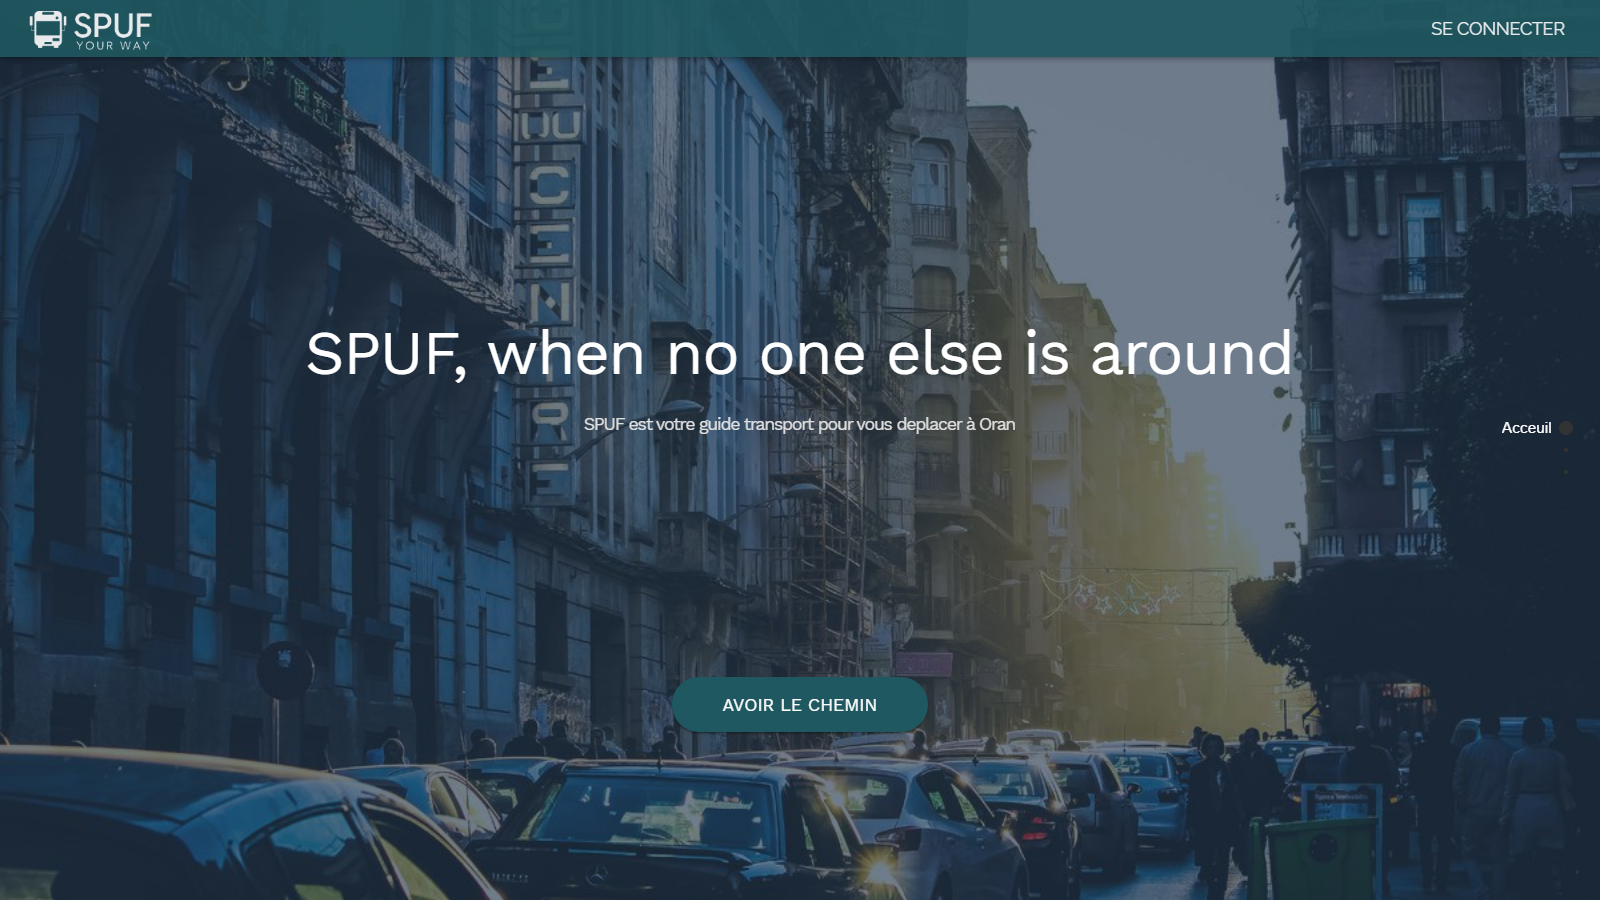
\includegraphics[width=\linewidth]{img/spuf/acceuil.png}
	 	\caption{Page d'accueil.}
	 \end{subfigure}
	 
	 \begin{subfigure}[b]{\linewidth}
	 	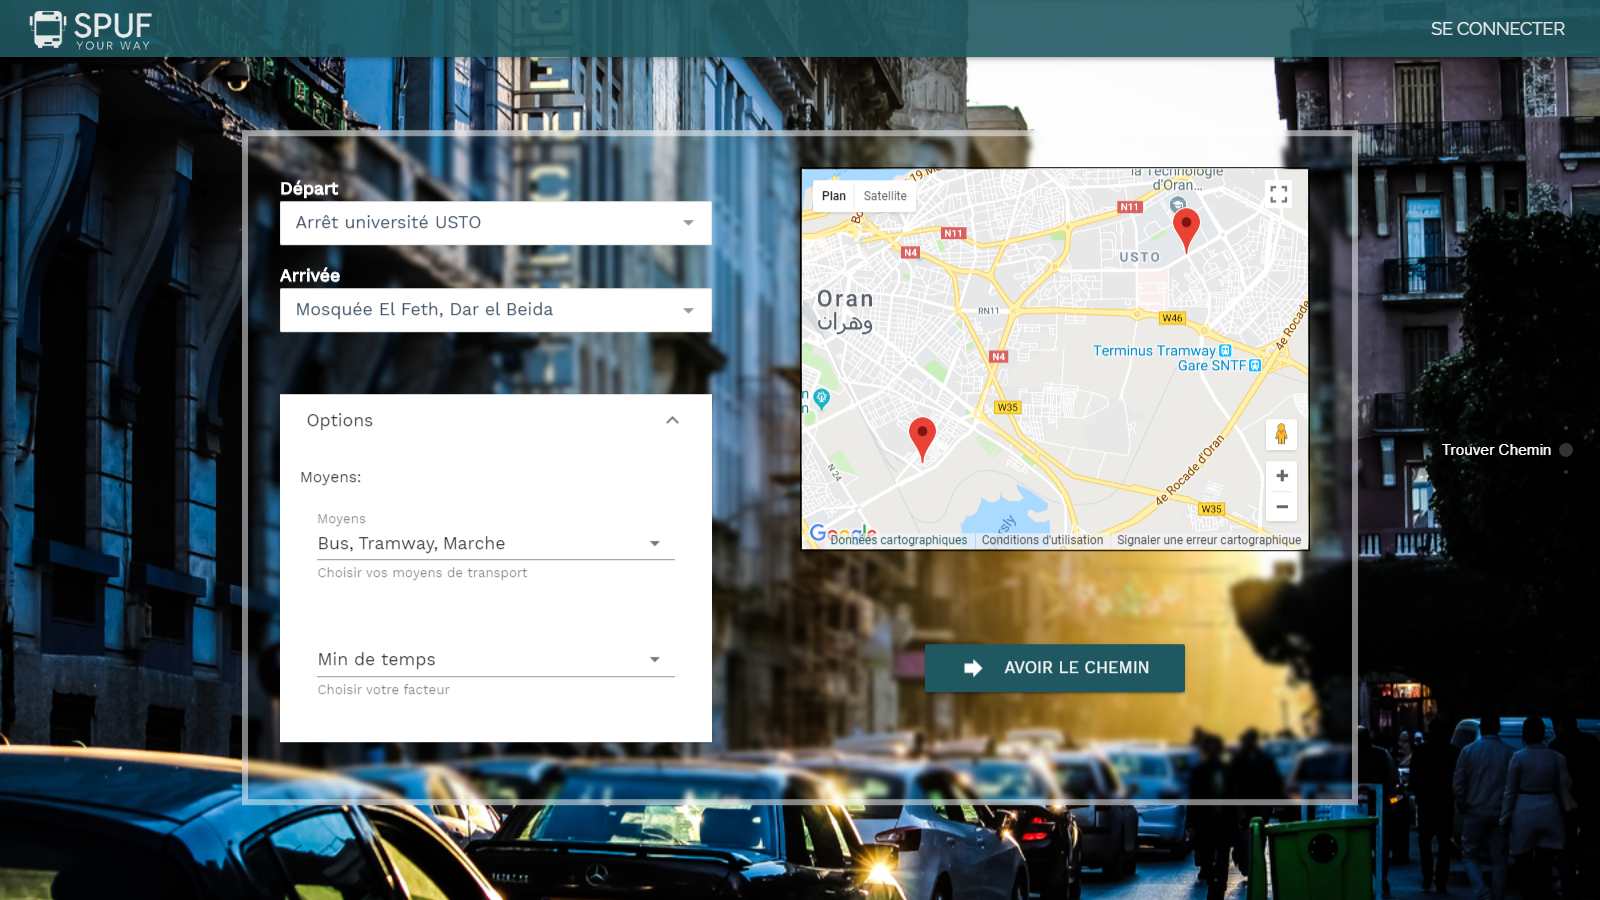
\includegraphics[width=\linewidth]{img/spuf/request.png}
	 	\caption{Page de requête.}	 
	 \end{subfigure}
	 
	\caption{Aperçu de l'application client.}
	 \label{fig:clientInterface}
\end{figure}


\begin{figure}
	 \begin{subfigure}[b]{\linewidth}
	 	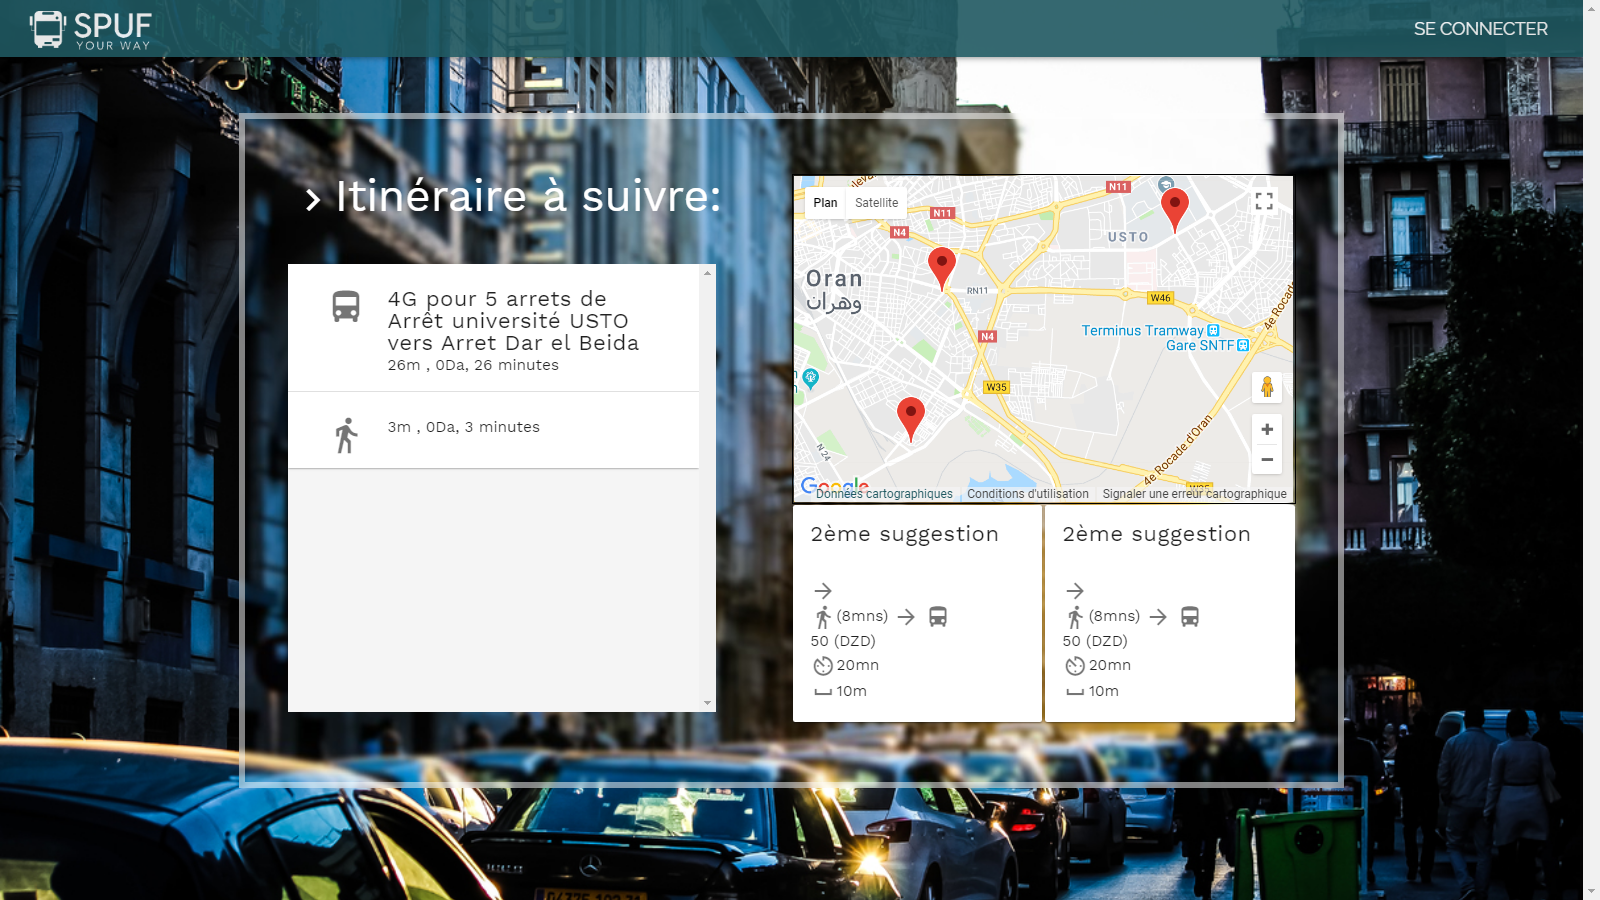
\includegraphics[width=\linewidth]{img/spuf/response.png}
	 	\caption{Page de réponse.}
	 \end{subfigure}
	 
	 \begin{subfigure}[b]{\linewidth}
	 	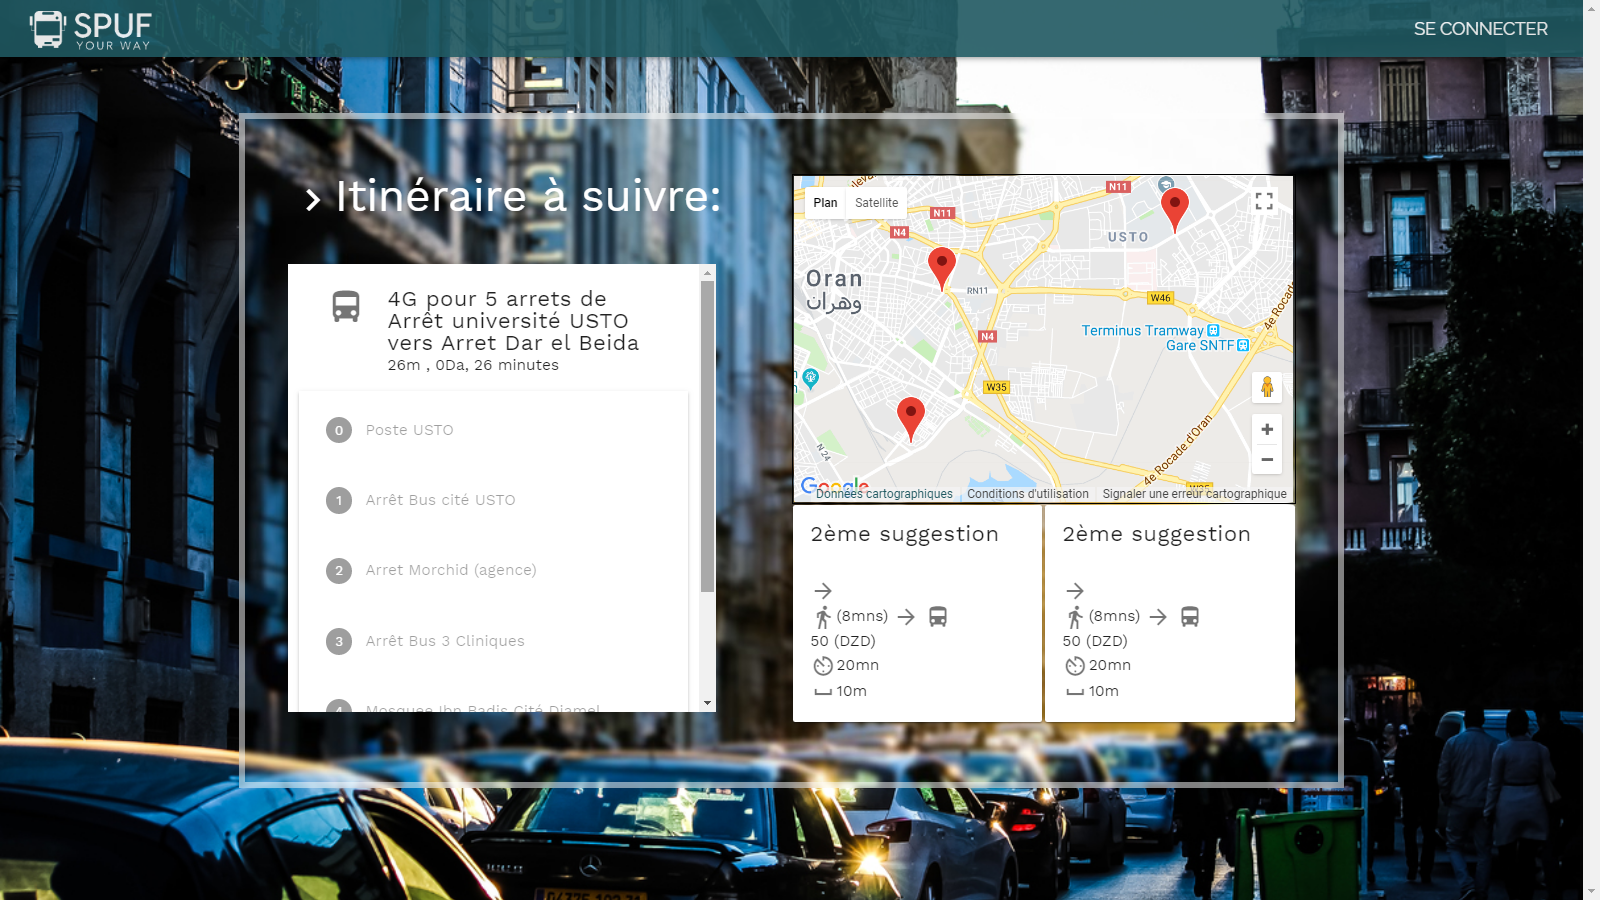
\includegraphics[width=\linewidth]{img/spuf/response2.png}
	 	\caption{Page de réponse détaillée.}	 
	 \end{subfigure}
	 \caption{Aperçu de l'application client.}
	 \label{fig:clientInterface2}
\end{figure}

\begin{figure}
	 \begin{subfigure}[b]{\linewidth}
	 	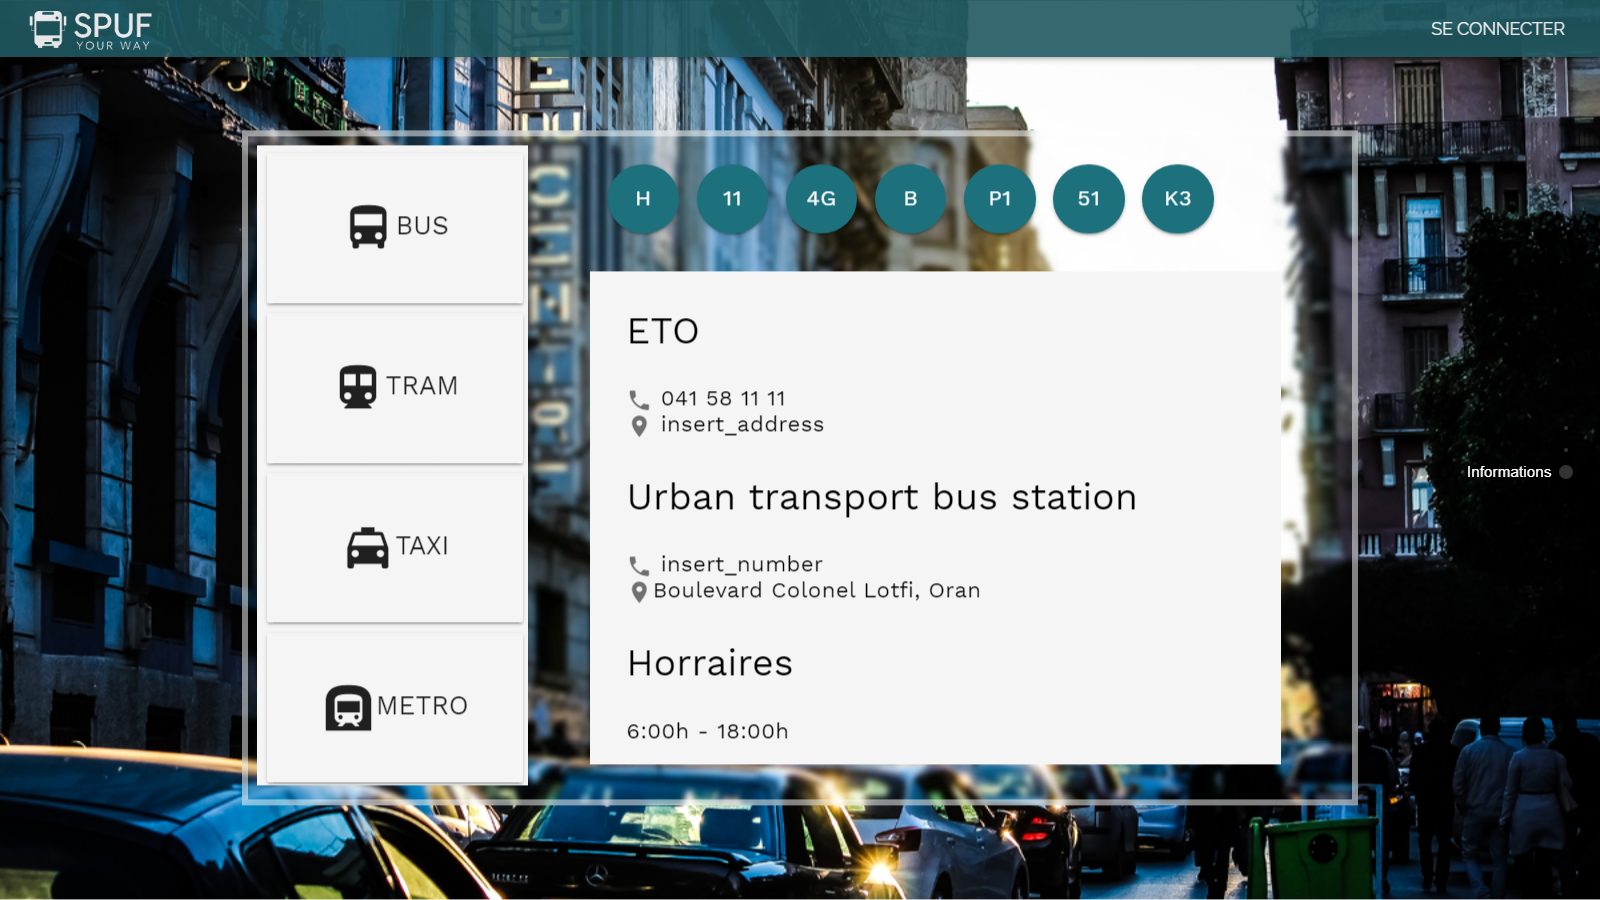
\includegraphics[width=\linewidth]{img/spuf/infobus.png}
	 	\caption{Page d'informations (bus).}
	 \end{subfigure}
	 
	 \begin{subfigure}[b]{\linewidth}
	 	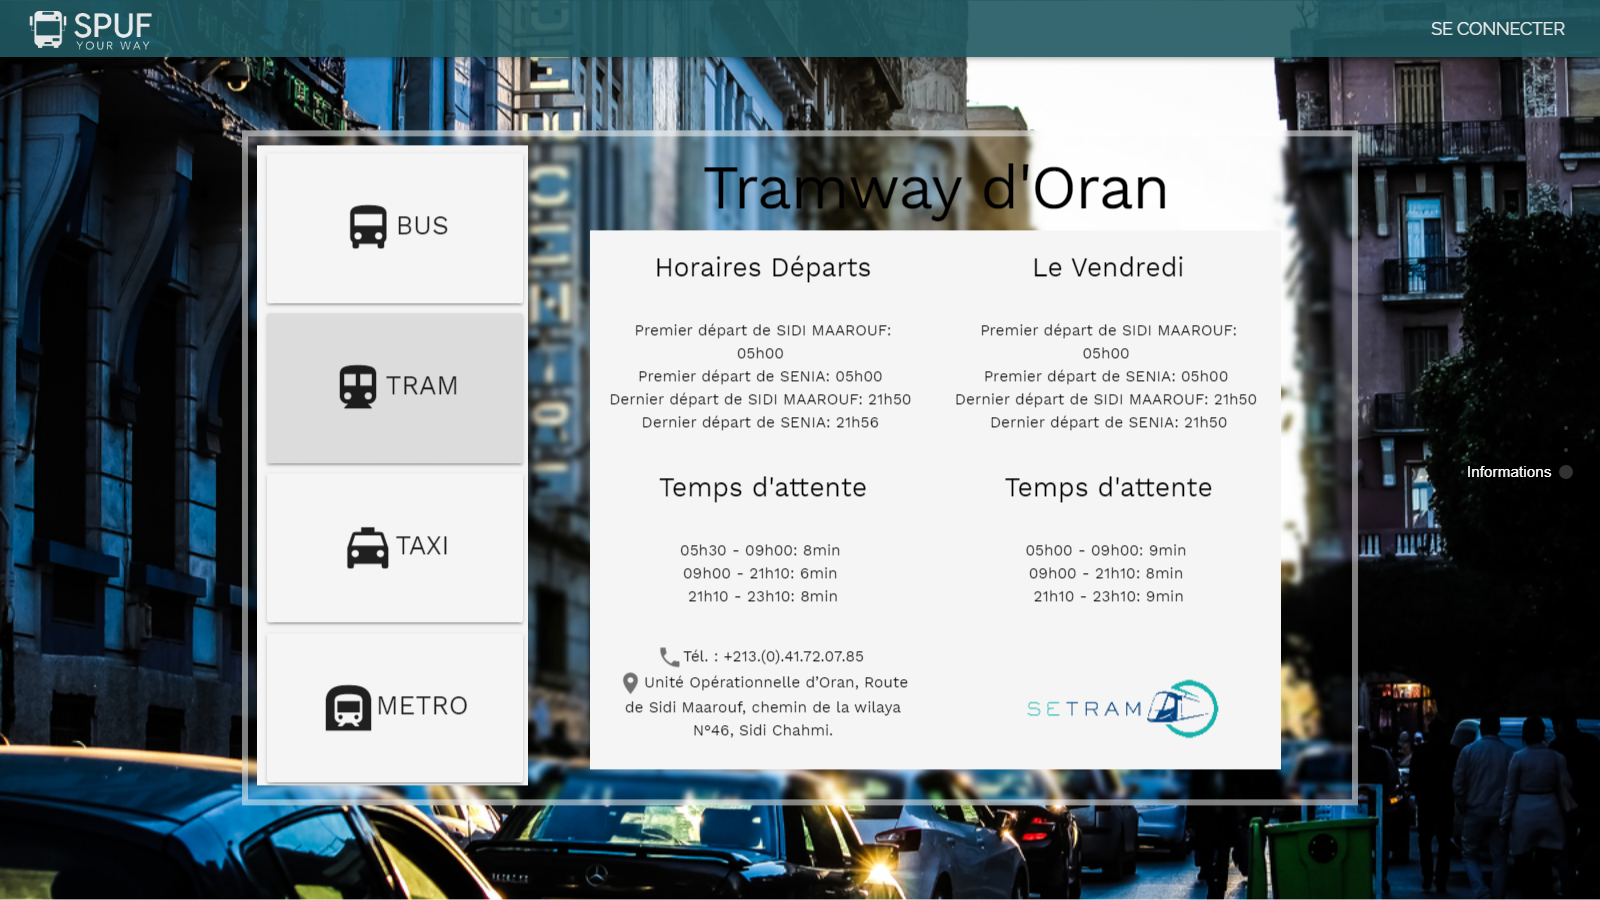
\includegraphics[width=\linewidth]{img/spuf/infotram.png}
	 	\caption{Page d'informations (Tramway).}	 
	 \end{subfigure}
	 \caption{Aperçu de l'application client.}
	 \label{fig:clientInterface3}
\end{figure}

\subsection{Application administrateur}
La partie administrateur consiste en une application web indépendante de l'application client, elle permet d'introduire de nouvelles stations et lignes avec les différentes informations de chacune.
Elle peut être complétée en ajoutant d'autres menus pour différents transports par exemple ou plus de fonctionnalités permettant d'ajouter plus facilement un grand nombre d'informations.\newline
Les interfaces de l'application administrateur sont donnés dans les figures \ref{fig:adminInterface} et \ref{fig:adminInterface2}.
\begin{figure}[h!]
	 \begin{subfigure}[b]{\linewidth}
	 	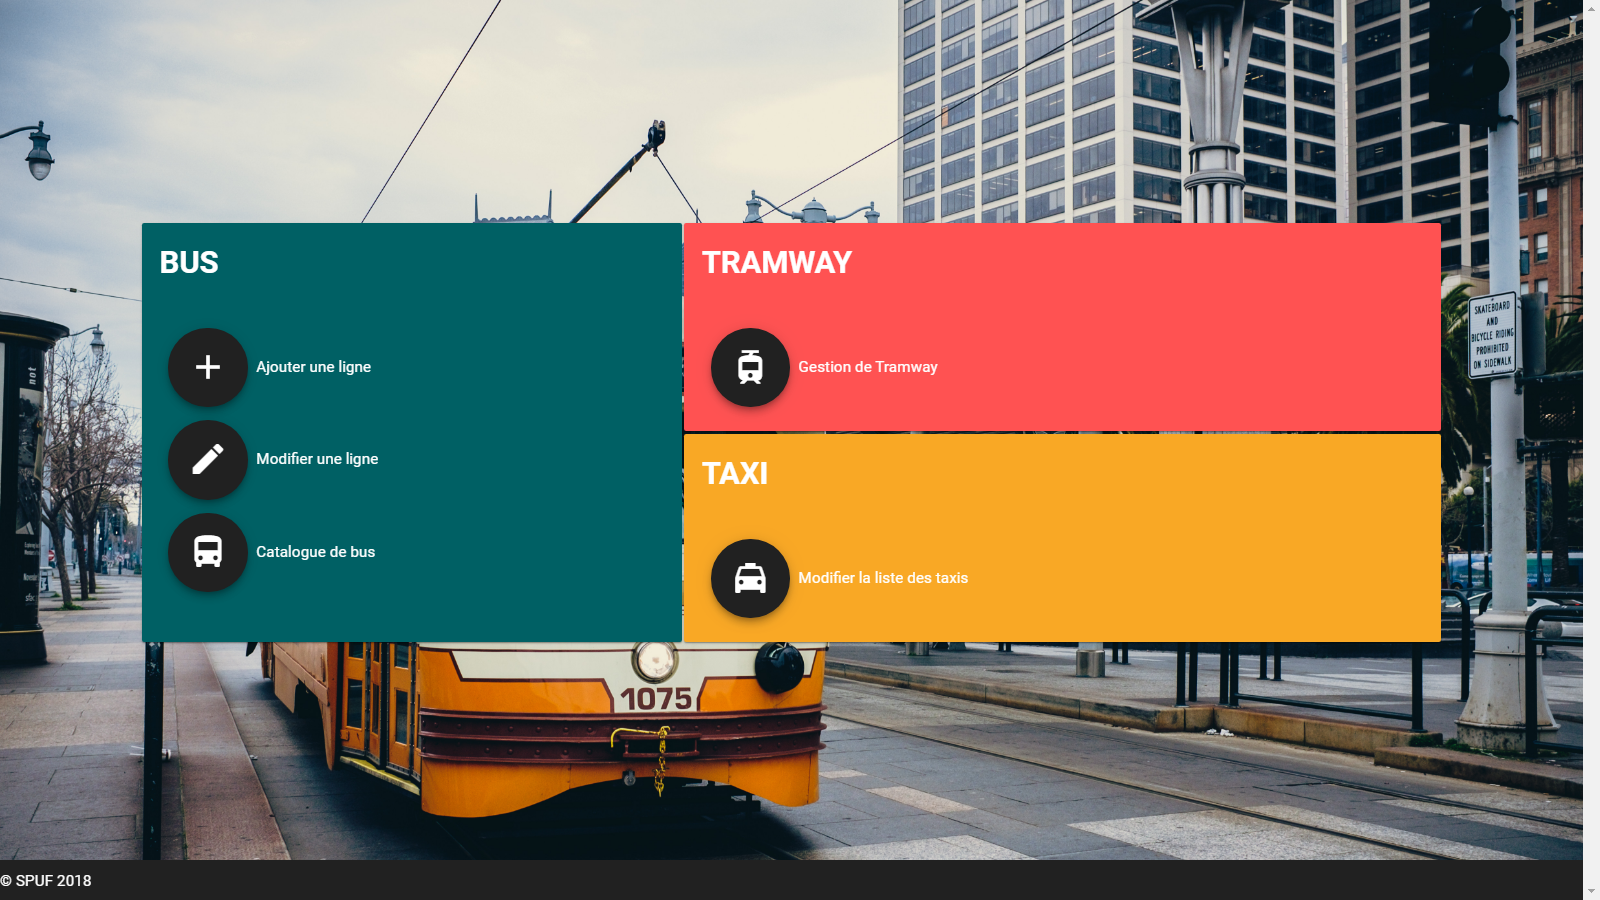
\includegraphics[width=\linewidth]{img/spuf/adminmenu.png}
	 	\caption{Page acceuil.}
	 \end{subfigure}
	 
	 \begin{subfigure}[b]{\linewidth}
	 	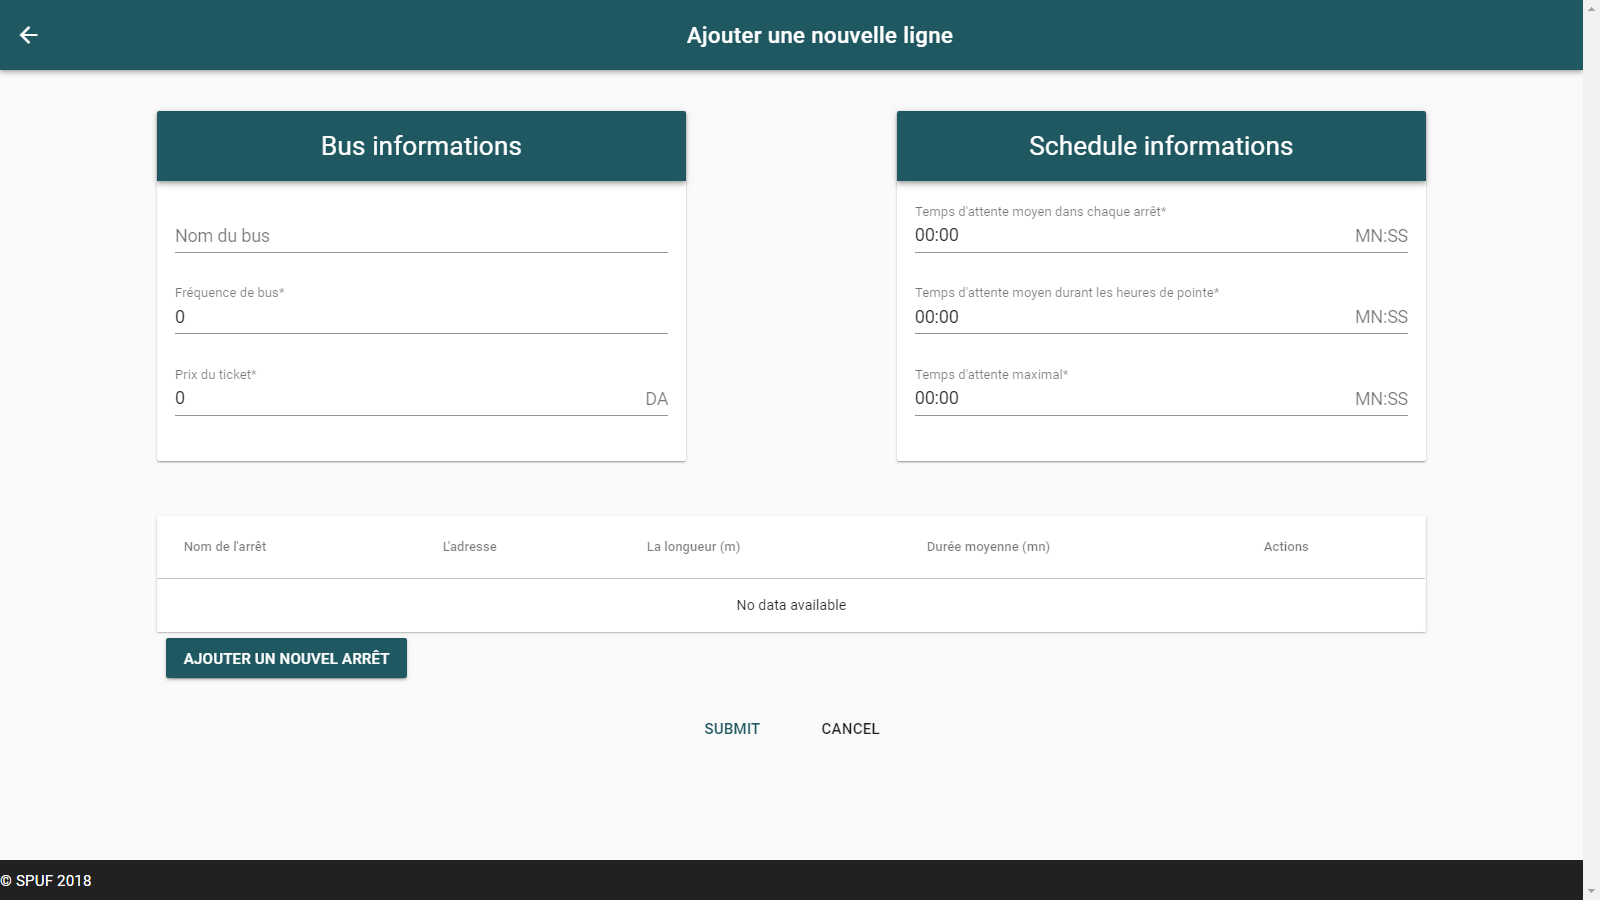
\includegraphics[width=\linewidth]{img/spuf/addline.png}
	 	\caption{Page ajout de nouvelles lignes.}
	 \end{subfigure}
	 \caption{Aperçu de l'application administrateur.}
	 \label{fig:adminInterface}
\end{figure}

\begin{figure}[h!]
	 \begin{subfigure}[b]{\linewidth}
	 	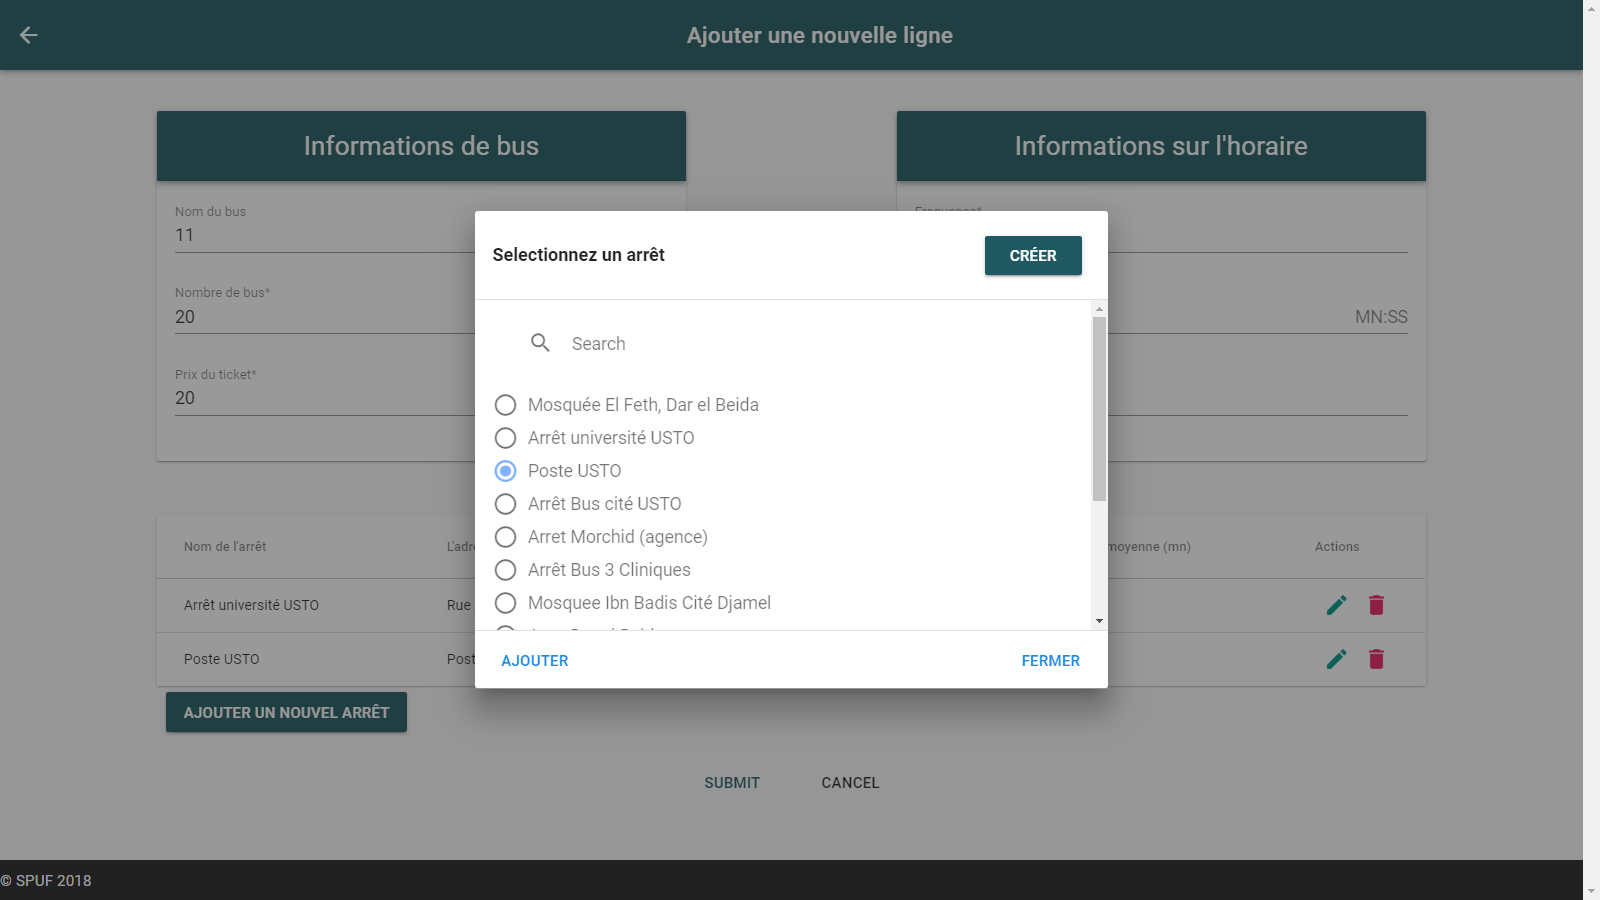
\includegraphics[width=\linewidth]{img/spuf/stationadd.png}
	 	\caption{Page ajout de nouvelles lignes.}	 
	 \end{subfigure}
	 
	 \begin{subfigure}[b]{\linewidth}
	 	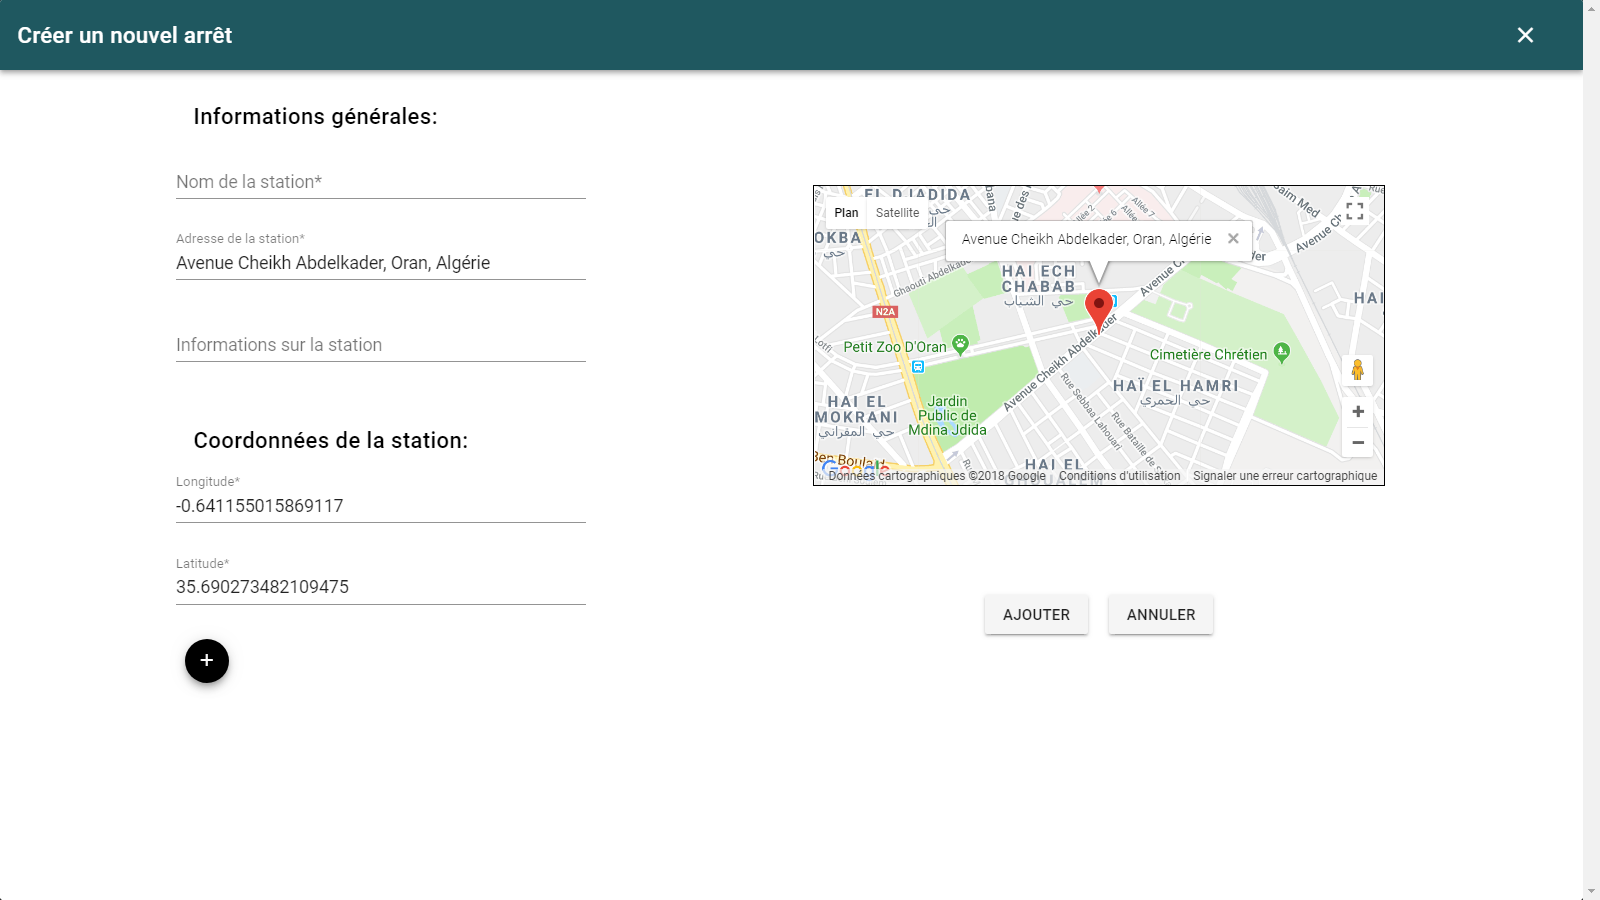
\includegraphics[width=\linewidth]{img/spuf/createstation.png}
	 	\caption{Page ajout de nouvelle station.}	 
	 \end{subfigure}
	 \caption{Aperçu de l'application administrateur.}
	 \label{fig:adminInterface2}
\end{figure}
%Chapitre 5
\chapter{Conclusion}
Evaluer le résultat 


\printbibliography[heading=bibintoc]

\end{document}